% !TEX root = userguide_en.tex
%----------------------------------------------------------
\chapter{File specification}
\label{Ch:HowToStandard}
%----------------------------------------------------------
\section{Input files for {\it Standard} mode}

% !TEX root = userguide_en.tex
%----------------------------------------------------------
An example of input file for the standard mode is shown below:

\begin{minipage}{10cm}
\begin{screen}
\begin{verbatim}
W = 2
 L = 4
 model = "spin"
 method = "Lanczos"

 lattice = "triangular lattice"
//mu = 1.0
// t = -1.0
// t' = -0.5
// U = 8.0
//V = 4.0
//V'=2.0
J = -1.0
J'=-0.5
// nelec = 8
2Sz = 0
\end{verbatim}
\end{screen}
\end{minipage}
~\\
~\\
~\\
{\bf Basic rules for input files}
\begin{itemize}
\item In each line, there is a set of a keyword (before an ``\verb|=|") and a parameter(after an ``\verb|=|"); 
  they are separated by ``\verb|=|".
\item You can describe keywords in a random order.
\item Empty lines and lines beginning in a ``\verb|//|''(comment outs) are skipped.
\item Upper- and lowercase are not distinguished.
  Double quotes and blanks are ignored.
\item There are three kinds of parameters.\\ 
  1.~Parameters that must be specified~(if not, $\HPhi$ will stop with error messages),\\ 
  2.~Parameters that is not necessary be specified~(if not, default values are used),\\
  3.~Parameters that must not be specified~(if specified, $\HPhi$ will stop with error messages).\\
  An example of 3 is transfer $t$ for the Heisenberg spin system. 
  If you choose ``model=spin", you should not specify ``$t$".
\end{itemize}

We explain each keywords as follows:

\subsection{Parameters about the kind of a calculation}

\begin{itemize}

\item \verb|model|

{\bf Type :} String (Choose from \verb|"Fermion Hubbard"|, \verb|"Spin"|, \verb|"Kondo Lattice"|, 
\verb|"Fermion HubbardGC"|, \verb|"SpinGC"|, \verb|"Kondo LatticeGC"|, \verb|"SpinGCBoost"|)
\footnote{GC=Grand Canonical}

{\bf Description :} The target model is specified with this parameter;
above words denote the canonical ensemble of the Fermion in the Hubbard model
\begin{align}
H = -\mu \sum_{i \sigma} c^\dagger_{i \sigma} c_{i \sigma} 
- \sum_{i \neq j \sigma} t_{i j} c^\dagger_{i \sigma} c_{j \sigma} 
+ \sum_{i} U n_{i \uparrow} n_{i \downarrow}
+ \sum_{i \neq j} V_{i j} n_{i} n_{j},
\label{fml4_1_hubbard}
\end{align}
canonical ensemble in the Spin model($\{\sigma_1, \sigma_2\}={x, y, z}$)
\begin{align}
H &= -h \sum_{i} S_{i z} + \Gamma \sum_{i} S_{i x} + D \sum_{i} S_{i z} S_{i z}
\nonumber \\
&+ \sum_{i j, \sigma_1}J_{i j \sigma_1} S_{i \sigma_1} S_{j \sigma_1}+ \sum_{i j, \sigma_1 \neq \sigma_2} J_{i j \sigma_1 \sigma_2} S_{i \sigma_1} S_{j \sigma_2} ,
\label{fml4_1_spin}
\end{align}
canonical ensemble in the Kondo lattice model
\begin{align}
H = - \mu \sum_{i \sigma} c^\dagger_{i \sigma} c_{i \sigma} 
- t \sum_{\langle i j \rangle \sigma} c^\dagger_{i \sigma} c_{j \sigma} 
+ \frac{J}{2} \sum_{i} \left\{
S_{i}^{+} c_{i \downarrow}^\dagger c_{i \uparrow}
+ S_{i}^{-} c_{i \uparrow}^\dagger c_{i \downarrow}
+ S_{i z} (n_{i \uparrow} - n_{i \downarrow})
\right\},
\label{fml4_1_kondo}
\end{align}
grand canonical ensemble of the Fermion in the Hubbard model [Eqn. (\ref{fml4_1_hubbard})],
grand canonical ensemble in the Spin model [Eqn. (\ref{fml4_1_spin})],
and
grand canonical ensemble in Kondo lattice model [Eqn. (\ref{fml4_1_kondo})]
respectively.

When \verb|model="SpinGCBoost"|,
by using more efficient algorithm\footnote{Y. Yamaji \textit{et. al.}, manuscript in preparation.}, 
$\HPhi$ calculates a system the same as \verb|"SpinGC"|.
However, supported models and MPI processes are highly limited.
See \verb|"Latice"| section.

\item \verb|method|
  
{\bf Type :} String (Choose from \verb|"Lanczos"|, \verb|"TPQ"|, \verb|"Full Diag"|)

{\bf Description :} The calculation type is specified with this parameter;
above words denote 
the single eigenstate calculation by using the Lanczos method,
at the finite-temperature by thermally pure quantum state,
and the full diagonalization method,
respectively.

\item \verb|lattice|

{\bf Type :} String (Choose from \verb|"Chain Lattice"|, \verb|"Square Lattice"|, 
\verb|"Triangular Lattice"|, \verb|Honeycomb Lattice|, \verb|Ladder|)

{\bf Description :} The lattice shape is specified with this parameter;
above words denote
the one dimensional chain lattice (Fig. \ref{fig_chap04_1_lattice}(a)), 
the two dimensional square lattice (Fig. \ref{fig_chap04_1_lattice}(b)),
the two dimensional triangular lattice (Fig. \ref{fig_chap04_1_lattice}(c)),
the two dimensional anisotropic honeycomb lattice (Fig. \ref{fig_chap04_1_honeycomb}),
the ladder lattice (Fig. \ref{fig_ladder}),
and
the Kagome Lattice(Only at \verb|method="SpinGCBoost"|. Fig. \ref{fig_kagome})
respectively.

In \verb|method="SpinGCBoost"|,
only \verb|"Chain Lattice"|, \verb|"Honeycomb Lattice"|, 
\verb|"Ladder"|, and \verb|"Kagome"| are supported.
Limits of $L$, $W$, and the number of MPI processes ($N_{\rm proc}$) are as follows:

\begin{itemize}

  \item \verb|"Chain Lattice"|

    $L = 8n$ (where $n$ is an integer number under the condition  $n\geq1$),
    $N_{\rm proc} \leq 2(L=8)$, $N_{\rm proc} \leq 2^{L/2-2}(L>8)$.
    
  \item \verb|"Honeycomb Lattice"|

    $W=3, L \geq 2$, $N_{\rm proc} \leq 2(L=2)$, $N_{\rm proc} \leq 64(L>2)$.

  \item \verb|"Ladder"|

    $W=2, L = 2n$ (where $n$ is an integer number under the condition  $n\geq4$),
    $N_{\rm proc} \leq 2^{L-4}$.

  \item \verb|"Kagome"|

    $W=3, L \geq 2$, $N_{\rm proc} \leq 1(L=2)$, $N_{\rm proc} \leq 512(L>2)$.

\end{itemize}

\begin{figure}[!htbp]
  \begin{center}
    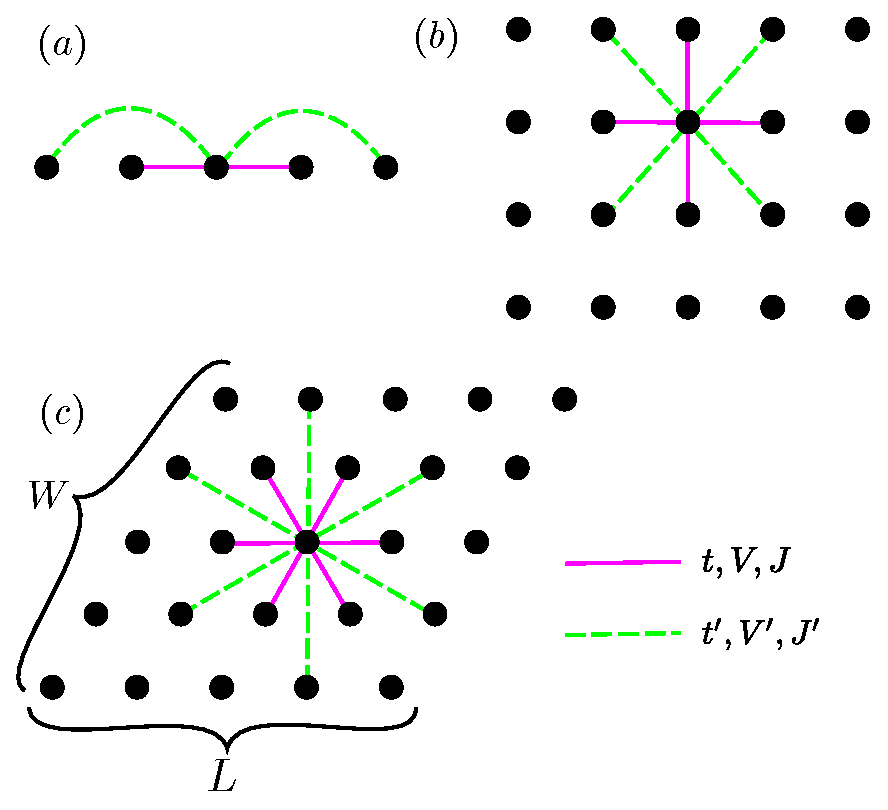
\includegraphics[width=8cm]{../figs/chap04_1_lattice.eps}
    \caption{Schematic illustration of
      (a) one dimensional chain lattice, 
      (b) two dimensional square lattice, and 
      (c) two dimensional triangular lattice.
      They have $t$, $V$, and $J$ as a nearest neighbor hopping, an offsite Coulomb integral, 
      and a spin-coupling constant, respectively (magenta solid lines);
      They also have $t'$, $V'$, and $J'$ as a next nearest neighbor hopping, offsite Coulomb integral, 
      and spin-coupling constant, respectively (green dashed line).
    }
    \label{fig_chap04_1_lattice}
  \end{center}
\end{figure}

\begin{figure}[!htbp]
  \begin{center}
    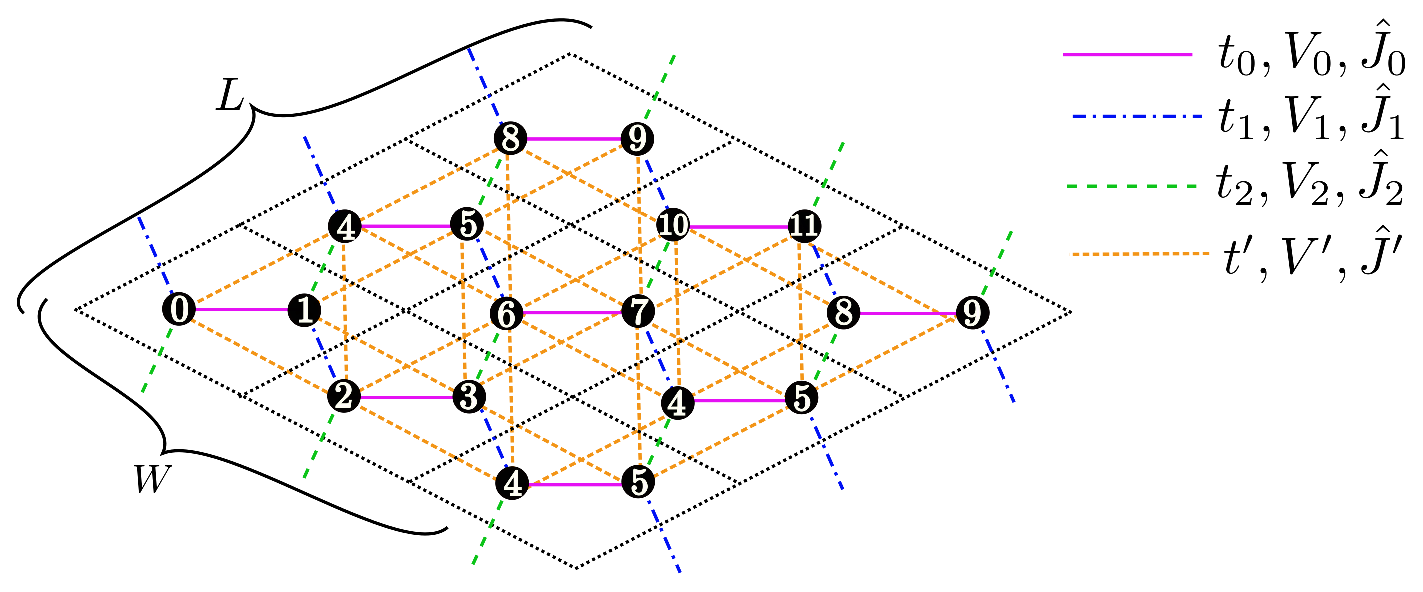
\includegraphics[width=15cm]{../figs/chap04_1_honeycomb.eps}
    \caption{Schematic illustration of the anisotropic honeycomb lattice.
      The nearest neighbor 
      hopping integral, spin coupling, offsite Coulomb integral
      depend on the bond direction.
      Those between second nearest neighbor sites are not supported.
    }
    \label{fig_chap04_1_honeycomb}
  \end{center}
\end{figure}

\begin{figure}[!htbp]
  \begin{center}
    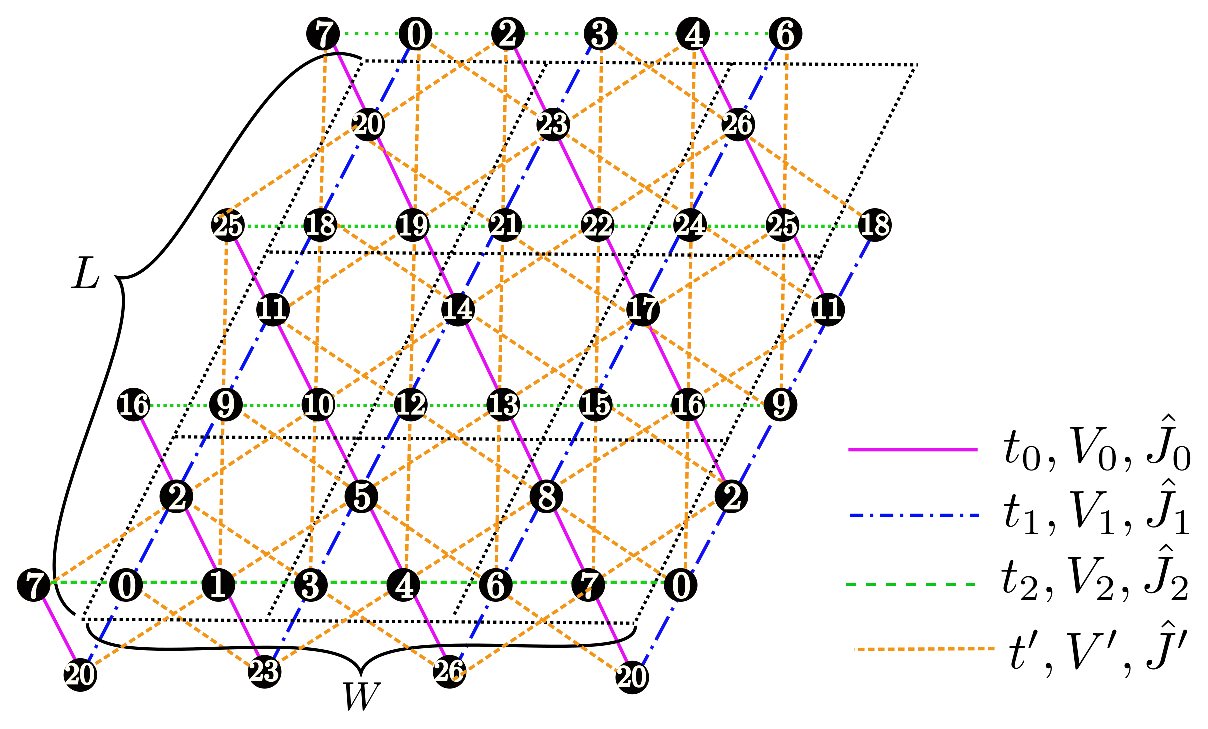
\includegraphics[width=10cm]{../figs/kagome.eps}
    \caption{Schematic illustration of the Kagome lattice.
    }
    \label{fig_kagome}
  \end{center}
\end{figure}

\begin{figure}[!htbp]
  \begin{center}
    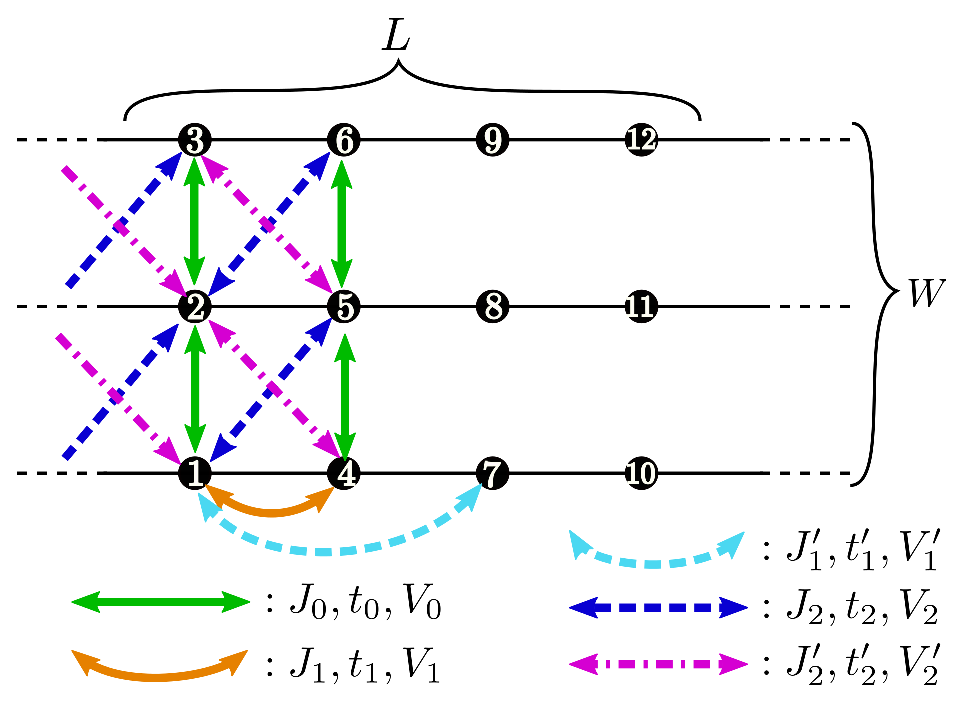
\includegraphics[width=10cm]{../figs/ladder.eps}
    \caption{Schematic illustration of the ladder lattice.
    }
    \label{fig_ladder}
  \end{center}
\end{figure}


\end{itemize}

\subsection{Parameters for the lattice}


\begin{figure}[!htbp]
  \begin{center}
    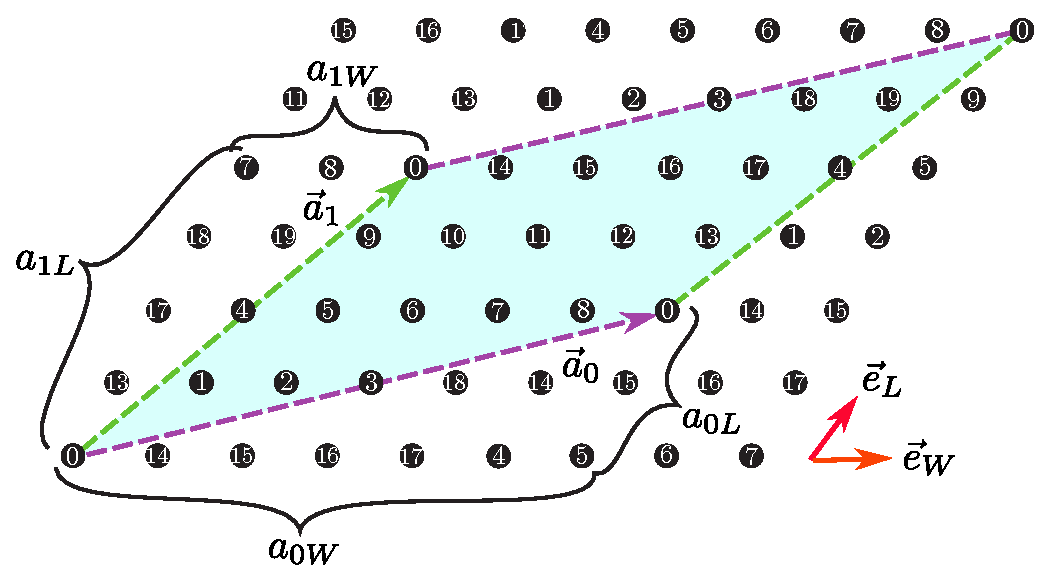
\includegraphics[width=8cm]{../figs/chap04_1_unitlattice.eps}
    \caption{Schematic illustration of a form of lattice where a pink and green vectors indicate first and second dimensional direction, respectively. 
    }
    \label{fig_chap04_1_unitlattice}
  \end{center}
\end{figure}

\begin{itemize}

\item \verb|a0L|

{\bf Type :} Positive integer ( 1.0 as a default)

{\bf Description :} The number of x-components of a vector defined as the first dimensional direction
is specified with this parameter  (Fig. \ref{fig_chap04_1_unitlattice}).

\item \verb|a0W|

{\bf Type :} Positive integer ( 0.0 as a default)

{\bf Description :} The number of y-components of a vector defined as the first dimensional direction
is specified with this parameter (Fig. \ref{fig_chap04_1_unitlattice}).

\item \verb|a1L|

{\bf Type :} Positive integer ( 0.0 as a default)

{\bf Description :} The number of x-components of a vector defined as the second dimensional direction
is specified with this parameter (Fig. \ref{fig_chap04_1_unitlattice}).

\item \verb|a1W|

{\bf Type :} Positive integer ( 1.0 as a default)

{\bf Description :} The number of y-components of a vector defined as the second dimensional direction
is specified with this parameter (Fig. \ref{fig_chap04_1_unitlattice}).


\item \verb|L|

{\bf Type :} Positive integer

{\bf Description :} The number of
sites along the first dimensional direction
is specified with this parameter.

\item \verb|W|

{\bf Type :} Positive integer

{\bf Description :} The number of
sites along the second dimensional direction
is specified with this parameter.
When \verb|lattice = "Chain Lattice"|, 
it should not be specified because it will not be used
(if specified, $\HPhi$ will stop).

\item \verb|a|

{\bf Type :} Real (\verb|1.0| as a default)

{\bf Description :} The lattice constant is specified with this parameter.
\end{itemize}

\subsection{Parameters for conserved quantities}

\begin{itemize}
\item \verb|nelec|

{\bf Type :} Positive integer

{\bf Description :} The number of valence electrons is specified with this parameter.
When \verb|model = "Fermion HubbardGC"|, \verb|"Spin"|, or  \verb|"SpinGC"|, 
it should not be specified.

\item \verb|2Sz|

{\bf Type :} Integer

{\bf Description :} The $z$ component of the twofold total spin is 
specified with this parameter.
When \verb|model = "Fermion HubbardGC"| or \verb|SpinGC|,
it should not be specified. 
\end{itemize}


\subsection{Parameters for each models}
A default value is set as $0$ unless a specific value is not defined in a description. Interactions are constructed by adding each interactions given by these parameters. Table~\ref{table_interactions} shows the parameters for each models. In the case of a complex type, a file format is ``{\it a real part, an imaginary part} " while in the case of a real type, only ``{\it a real part} ".

\begin{table}[hbp]
  \begin{tabular}{|l||c|c|c|c|c|c|c|c|} \hline
    Interactions & 1D chain & 2D square & 2D triangular & Honeycomb & Kagome & Ladder\\ \hline \hline
   \verb|J|, \verb|t|, \verb|V| & $\circ$	 & - 	& - 	& - 	& - 	& -\\ \hline
    \verb|J'|, \verb|t'|, \verb|V'| & $\circ$	 & $\circ$	& $\circ$ 	& $\circ$ 	& $\circ$ & - \\ \hline
   \verb|J0|, \verb|t0|, \verb|V0| & -	 & $\circ$ 	& $\circ$ 	& $\circ$ 	& $\circ$ & $\circ$\\ \hline
    \verb|J1|, \verb|t1|, \verb|V1| & -         	 & $\circ$ 	& $\circ$ 	& $\circ$ 	& $\circ$ & $\circ$\\ \hline
    \verb|J2|, \verb|t2|, \verb|V2|  & -         	 & -    	& $\circ$ 	& $\circ$ 	& $\circ$ & $\circ$\\ \hline
    \verb|J1'|, \verb|t1'|, \verb|V1'| & -		 &-	 	& -		& -		& -		& $\circ$ 	\\ \hline
    \verb|J2'| ,\verb|t2'|, \verb|V2'|  & -		 &-	 	& -		& -		& -		& $\circ$\\ \hline
    \verb|J3'|, \verb|t3'|, \verb|V3'|  & -		 &-	 	& -		& -		& -		& $\circ$\\ \hline
  \end{tabular}
   \caption{Interactions for each models defined in an input file. We can define spin couplings as matrix format.}
    \label{table_interactions}
\end{table}

\subsection{Parameters for the Hubbard model}
\begin{itemize}
\item \verb|mu|

{\bf Type :} Real

{\bf Description :} The chemical potential $\mu$ (including the site potential)
is specified with this parameter.

\item \verb|t|, \verb|t'|

{\bf Type :} Complex

{\bf Description :} The hopping (See Figs. \ref{fig_chap04_1_lattice}-\ref{fig_kagome})
is specified with this parameter.

\item \verb|t0|, \verb|t1|, \verb|t2|

{\bf Type :} Complex

{\bf Description :} The nearest neighbor hopping 
in the anisotropic honeycomb lattice 
(See Figs. \ref{fig_chap04_1_lattice}-\ref{fig_ladder})
is specified with this parameter.

\item \verb|t1'|,  \verb|t2'|, \verb|t3'|

{\bf Type :} Complex

{\bf Description :} Hopping integrals
in the ladder lattice 
(See Fig. \ref{fig_ladder})
is specified with this parameter.

\item \verb|U|

{\bf Type :} Real

{\bf Description :} The onsite Coulomb integral $U$ is specified with this parameter.

\item \verb|V|, \verb|V'|

{\bf Type :} Real

{\bf Description :} The nearest neighbor offsite Coulomb integrals $V$
and the second nearest neighbor offsite Coulomb integrals $V'$
(Fig. \ref{fig_chap04_1_lattice} are specified with these parameters.

\item \verb|V0|, \verb|V1|, \verb|V2|

{\bf Type :} Real

{\bf Description :} Nearest neighbor offsite Coulomb integrals 
on the anisotropic honeycomb lattice
(Fig. \ref{fig_chap04_1_honeycomb} are specified with these parameters.

\item \verb|V1'|, \verb|V2'|, \verb|V3'|

{\bf Type :} Real

{\bf Description :} Offsite Coulomb integrals 
on the ladder lattice
(Fig. \ref{fig_chap04_1_honeycomb} are specified with these parameters.

\end{itemize}

\subsection{Parameters for the Spin model}
\begin{itemize}
\item \verb|2S|

{\bf Type :} Positive integer (\verb|1| as a default)

{\bf Description :} The twofold moment of a localized spin is specified 
with this parameter (e. g. \verb|2S=1| for $1/2$ spin system). 

\item \verb|h|, \verb|Gamma|, \verb|D|

{\bf Type :} Real

{\bf Description :} The longitudinal magnetic field, transverse magnetic field, 
and the single-site anisotropy parameter are specified with these parameters.

\item \verb|J|, \verb|J'|, \verb|J|$\sigma_1$, \verb|J|$\sigma_1\sigma_2$,  \verb|J'|$\sigma_1$, \verb|J'|$\sigma_1\sigma_2$\\
  (\{${\sigma_1, \sigma_2}$\}=\{\verb|x|, \verb|y|, \verb|z|\} and ${\sigma_1\neq \sigma_2}$)

{\bf Type :} Real

{\bf Description :} The spin-coupling constant between nearest neighbor sites
(See Figs. \ref{fig_chap04_1_lattice}-\ref{fig_kagome}) is specified with this parameter.

\item \verb|J0|, \verb|J1|, \verb|J2|, \verb|J0|$\sigma_1$, \verb|J1|$\sigma_1$, \verb|J2|$\sigma_1$,
 \verb|J0|${\sigma_1\sigma_2}$, \verb|J1|${\sigma_1\sigma_2}$, \verb|J2|${\sigma_1\sigma_2}$ \\
  (\{${\sigma_1, \sigma_2}$\}=\{\verb|x|, \verb|y|, \verb|z|\} and ${\sigma_1\neq \sigma_2}$)

{\bf Type :} Real

{\bf Description :} Spin-coupling constants between nearest neighbor sites
in the anisotropic honeycomb lattice
(See Figs. \ref{fig_chap04_1_lattice}-\ref{fig_ladder}) are specified with these parameter.

\item \verb|J1'|,\verb|J2'|,\verb|J3'|,  \verb|J1'|$\sigma_1$, \verb|J2'|$\sigma_1$, \verb|J3'|$\sigma_1$,
\verb|J1'|${\sigma_1\sigma_2}$, \verb|J2'|${\sigma_1\sigma_2}$, \verb|J3'|${\sigma_1\sigma_2}$\\
 (\{${\sigma_1, \sigma_2}$\}=\{\verb|x|, \verb|y|, \verb|z|\} and ${\sigma_1\neq \sigma_2}$)

{\bf Type :} Real

{\bf Description :} Spin-coupling constants in the ladder lattice
(See Fig. \ref{fig_ladder}) are specified with these parameter.

\end{itemize}

\subsection{Parameters for the Kondo model}
\begin{itemize}
\item \verb|mu|

{\bf Type :} Real

{\bf Description :} The chemical potential $\mu$ (including the site potential)
is specified with this parameter.

\item \verb|t|, \verb|t'|

{\bf Type :} Complex

{\bf Description :} The hopping (See Figs. \ref{fig_chap04_1_lattice}-\ref{fig_kagome})
is specified with this parameter.

\item \verb|t0|, \verb|t1|, \verb|t2|

{\bf Type :} Complex

{\bf Description :} The nearest neighbor hopping 
in the anisotropic honeycomb lattice 
(See Figs. \ref{fig_chap04_1_lattice}-\ref{fig_ladder})
is specified with this parameter.

\item \verb|t1'|,  \verb|t2'|, \verb|t3'|

{\bf Type :} Complex

{\bf Description :} Hopping integrals
in the ladder lattice 
(See Fig. \ref{fig_ladder})
is specified with this parameter.

\item \verb|J|

{\bf Type :} Real(\verb|0.0| as a default)

{\bf Description :} The spin-coupling constant between the valence and the local electrons
is specified with this parameter.

\end{itemize}

\subsection{Parameters for the numerical condition}
\begin{itemize}
\item \verb|Lanczos_max|

{\bf Type :} Positive integer (\verb|2000| as a default)

{\bf Description :} Upper limit of the Lanczos step is specified with this parameter.

\item \verb|initial_iv|

{\bf Type :} Integer (\verb|-1| as a default)

{\bf Description :} 
{An initial vector is specified with this parameter.}
\begin{itemize}
\item{Lanczos method}
\begin{itemize}
\item{For canonical ensemble and \verb|initial_iv| $\geq 0$}

The non-zero components of an initial vector is specified with this parameter. 

\item{For grand canonical ensemble or \verb|initial_iv| $< 0$}

A seed of random generator is given by this parametar and the random vector is used as an initial vector.
\end{itemize}

\item{TPQ method}

A seed of random generator is given by this parametar and the random vector is used as an initial vector.
\end{itemize}
See \ref{Ch:algorithm} for details of setting an initial vector.

\item \verb|nvec|

{\bf Type :} Positive integer (\verb|1| as a default)

{\bf Description :} We specify the number of getting 
eigenvalues from the ground energy by Lanczos method.\\
When nvec=2, we obtain the ground-state energy and energy of the first-excited state.

\item \verb|exct|

{\bf Type :} Positive integer (\verb|1| as a default)

{\bf Description :}  We specify the number of getting eigenvectors from the ground energy by Lanczos method.\\
When exct=2, we obtain the eigenvector of the first-excited state.

{\bf Note}:  the following condition must be satisfied: \verb|nvec| $>=$ \verb|exct|.

\item \verb|LanczosEps|

{\bf Type :} Positive Integer (\verb|14| as a default)

{\bf Description :} The convergence criteria for the Lanczos method is specified with this parameter.
If the difference between the old and the new target eigenvalue fall below $10^{- \verb|LanczosEps|}$, 
the Lanczos step will finish.

\item \verb|LancczosTarget|

{\bf Type :} Positive integer (\verb|2| as a default)

{\bf Description :} We specify the target eigenenergy for the convergence criteria.
If this set to \verb|1|, target eigenenergy becomes the ground state.

\item \verb|LargeValue|

{\bf Type :} Double (The default value is written below.)

{\bf Description :} (Only for TPQ) 
We use $l$ as $l-\hat{H}/N_{s}$ in the TPQ calculation.
Usually, the largest eigenvalue of Hamiltonian is used as $l$. 
Thus, we take the default value of $l$ for each models is as follows:

\begin{itemize}

\item Hubbard model [Eqn. (\ref{fml4_1_hubbard})]

The canonical ensemble
\begin{align}
l = |\mu| \frac{N_{\rm elec}}{N_{\rm site}}
+ 2 z |t| + 2 z' |t'| + |U| + 2 z |V| + 2 z' |V'| 
\end{align}
The grand canonical ensemble
\begin{align}
l = 2|\mu|
+ 2 z |t| + 2 z' |t'| + |U| + 2 z |V| + 2 z' |V'|
\end{align}

\item Spin model [Eqn. (\ref{fml4_1_spin})]

The canonical ensemble
\begin{align}
l = \frac{|S_z^{\rm tot}|}{N_{\rm site}}|h| + S |\Gamma| + S^2 |D|
+\frac{z}{2} S^2 (|J_x|+|J_y|+|J_z|) +\frac{z'}{2} S^2 (|J'_x|+|J'_y|+|J'_z|)
\end{align}
The grand canonical ensemble
\begin{align}
l = S |h| + S |\Gamma| + S^2 |D|
+\frac{z}{2} S^2 (|J_x|+|J_y|+|J_z|) + \frac{z'}{2} S^2 (|J'_x|+|J'_y|+|J'_z|) 
\end{align}

\item Kondo lattice model [Eqn. (\ref{fml4_1_kondo})]

The canonical ensemble
\begin{align}
l = |\mu| \frac{N_{\rm elec}}{N_{\rm site}} + 2 z |t| + \frac{S}{2} |J| 
\end{align}
The grand canonical ensemble
\begin{align}
l = 2|\mu| + 2 z |t| + \frac{S}{2} |J| 
\end{align}

\end{itemize}

\item \verb|NumAve|

{\bf Type :} Positive integer (\verb|5| as a default)

{\bf Description :} (Only for the TPQ) The number of independent runs for the TPQ method is specified 
with this parameter.

\item \verb|ExpecInterval|

{\bf Type :} Positive integer (\verb|20| as a default)

{\bf Description :} (Only for the TPQ) 
We specify the interval steps of calculating correlation functions in TPQ method.\\ 
{\bf Note:} The small interval increases the time cost of calculations.

\end{itemize}

\section{Input files for {\it Expert} mode}
\label{Ch:HowToExpert}
In this section, details of input files for expert mode are explained. Input files are categorized by the following four parts.
\begin{description}
\item[(1)~List:] This file is a list of input file names with keywords. Each keywords is fixed, but file names are free to be determined.  
\item[(2)~Basic parameters:] The following input files give basic parameters. 
The kinds of input files are determined by keywords. 
~\\{\bf CalcMod}: Set the parameters for calculation modes.
~\\{\bf ModPara}: Set the parameters for basic parameters such as site number, electron number, Lanczos step {\it etc}.
~\\{\bf LocSpin}: Set the location of local spin (only used in Kondo model). 
\item[(3)~Hamiltonian:] 
Hamiltonian for $\HPhi$ is denoted by the format of interactions for electron system. 
The kinds of interactions are determined by the following keywords. 
~\\{\bf Trans}: The one body part, $c_{i\sigma_1}^{\dag}c_{j\sigma_2}$.
~\\{\bf InterAll}: The general two body interactions, $c_ {i \sigma_1}^{\dag}c_{j\sigma_2}c_{k \sigma_3}^{\dag}c_{l \sigma_4}$.
~\\We can set interactions which are often used by the following keywords. 
~\\{\bf CoulombIntra}: On-site Coulomb interactions, $n_ {i \uparrow}n_{i \downarrow}$ ($n_{i \sigma}=c_{i\sigma}^{\dag}c_{i\sigma}$).
~\\{\bf CoulombInter}: Off-site Coulomb interactions, $n_ {i}n_{j}$ ($n_i=n_{i\uparrow}+n_{i\downarrow}$).
~\\{\bf Hund}: Hund couplings, $n_{i\uparrow}n_{j\uparrow}+n_{i\downarrow}n_{j\downarrow}$.
~\\{\bf PairHop}: Pair hopping couplings, $c_ {i \uparrow}^{\dag}c_{j\uparrow}c_{i \downarrow}^{\dag}c_{j  \downarrow}$.
~\\{\bf Exchange}: Exchange couplings, $c_ {i \uparrow}^{\dag}c_{j\uparrow}c_{j \downarrow}^{\dag}c_{i  \downarrow}$.
~\\{\bf Ising}: Ising interactions, $S_i^z S_j^z$.
~\\{\bf PairLift}: PairLift couplings, $c_ {i \uparrow}^{\dag}c_{i\downarrow}c_{j \uparrow}^{\dag}c_{j \downarrow}$.
\item[(4)~Output:] Targets for output is determined.
~\\{\bf OneBodyG }: One-body green functions,  $\langle c^{\dagger}_{i\sigma_1}c_{j\sigma_2}\rangle$.
~\\{\bf TwoBodyG }: Two-body green functions,  $\langle c^{\dagger}_{i\sigma_1}c_{j\sigma_2}c^{\dagger}_{k \sigma_3}c_{l\sigma_4}\rangle$.
\end{description}

~\subsection{List file for Input files}
\label{Subsec:InputFileList}.
This file determines input filenames which are correlated with keywords. File format is shown as follows.\\
\begin{minipage}{10cm}
\begin{screen}
\begin{verbatim}
CalcMod  calcmod.def
ModPara  modpara.def
LocSpin  zlocspn.def
Trans    ztransfer.def
InterAll zinterall.def
OneBodyG zcisajs.def
TwoBodyG	zcisajscktaltdc.def
\end{verbatim}
\end{screen}
\end{minipage}
\\
\subsubsection{File format}
[string01]~[string02]
\subsubsection{Parameters}
 \begin{itemize}
   \item  $[$string01$]$
   
   {\bf Type :} string-type
   
   {\bf Description :} Select a word from keywords.
   
   \item  $[$string02$]$
   
    {\bf Type :} string-type 

   {\bf Description :} An input filename which is correlated with keywords.
 \end{itemize}
\subsubsection{Use rules}
\begin{itemize}
\item  After setting keywords at [string 01], half-width state is needed for writing a filename. You can set the filename freely.
\item Keywords for input files are shown in Table\ref{Table:Defs}.
\item Essential keywords are ``CalcMod", ``ModPara" and ``LocSpin".
\item Keywords can be set in random order.
\item If keywords or filenames are incorrect, the program is terminated. 
\item When the head of line is ``$\#$", the line is skipped.
\end{itemize}

 \begin{table*}[h!]
\begin{center}
  \begin{tabular}{ll|} \hline
           Keywords     & Details for corresponding files       \\   \hline\hline
           CalcMod      &   Parameters for modes of calculation.  \\  \hline  
           ModPara       &  Parameters for calculation.        \\ \hline   
           LocSpin         &  Configurations of the local spins for Hamiltonian.         \\ 
           Trans       &   Transfer and chemical potential for Hamiltonian.  \\
           InterAll  &   Two-body interactions for Hamiltonian. \\  
           CoulombIntra  &   CoulombIntra interactions. \\  
           CoulombInter  &   CoulombInter  interactions. \\  
           Hund  &   Hund couplings. \\  
           PairHop  &  Pair hopping couplings. \\  
           Exchange  &  Exchange couplings. \\  
           Ising  &  Ising interactions. \\  
           PairLift  &   Pair lift couplings. \\  
           OneBodyG         &   Output components for Green functions $\langle c_{i\sigma}^{\dagger}c_{j\sigma}\rangle$           \\   
           TwoBodyG &   Output components for Correlation functions $\langle c_{i\sigma}^{\dagger}c_{j\sigma}c_{k\tau}^{\dagger}c_{l\tau}\rangle$  \\   \hline
  \end{tabular}
\end{center}
\caption{List of the definition files.}
\label{Table:Defs}
\end{table*}%

\newpage
%----------------------------------
\subsection{CalcMod file}
\label{Subsec:calcmod}
This file determines parameters for calculation method, model and output mode. File format is shown as follows.\\
\begin{minipage}{10cm}
\begin{screen}
\begin{verbatim}
CalcType   0
CalcModel   2
CalcEigenVec 0
\end{verbatim}
\end{screen}
\end{minipage}
\\
%----------------------------------
\subsubsection{File format}
[string01]~[int01]
\subsubsection{Parameters}
 \begin{itemize}
   \item  $[$string01$]$
   
   {\bf Type :} string-type
   
   {\bf Description :} Select a word from keywords.
   
   \item  $[$int01$]$
   
    {\bf Type :} int-type 

   {\bf Description :} A parameter which is correlated with a keyword.\\

   
  \end{itemize}

\subsubsection{Use rules}
\begin{itemize}
\item After setting keywords at [string 01], a half-width blank is needed for setting a parameter.
\item Keywords can be set in random order.
\item If keywords or filenames are incorrect, the program is terminated. 
\item The following keywords, ``CalcType" and ``CalcModel" are essential. 
\item When the head of line is ``$\#$", the line is skipped.
\end{itemize}
~\subsubsection{Keywords and parameters}
Parameters correlated with keywords are shown as follows.
\begin{itemize}
\item  \verb|CalcType|

{\bf Type :} int-type 

{\bf Description :} Select the method for calculation from the following list:\\
0: Lanczos method,\\
1: Analysis of the physical properties by using TPQ,\\
2: Full diagonalization method.\\

\item  \verb|CalcModel|

{\bf Type :} int-type 

{\bf Description :} Select the model from the following list:\\
0: fermion Hubbard model (Canonical ensemble: conservation of particles, the component of $S_z$)\\
1: Spin model (Canonical ensemble: conservation of the component of $S_z$)\\
2: Kondo lattice model (Canonical ensemble: conservation of particles, the component of $S_z$)\\
3: fermion Hubbard model (Grand canonical ensemble)\\
4: Spin model (Grand canonical ensemble)\\
5: Kondo lattice model (Grand canonical ensemble)

%\item  \verb|Outputmode|
%
%{\bf Type :} int-type (default value: 0)
%
%{\bf Description :} Select the output mode from the following list:\\
%0: Output of Green's function. The components are set by the OneBodyG and TwoBodyG input files.\\
%1: Output of charge correlation function, spin correlation function and Green's function (not supported in ver.0.1). The components of Green's function are set by the OneBodyG and TwoBodyG input files.\\

\item  \verb|CalcEigenVec|

{\bf Type :} int-type (default value: 0)

{\bf Description :} Select the method to calculate eigenvectors:\\
0:Lanczos+CG methods (When the convergence of eigenvectors are not enough for using Lanczos method,  CG method is applied to calculate eigenvectors).\\
1:Lanczos method.\\

\item  \verb|InitialVecType|

{\bf Type :} int-type (default value: 0)

{\bf Description :} Select the type of an initial vector:\\
0:Complex type.\\
1:Real type.\\

\item  \verb|OutputEigenVec|

{\bf Type :} int-type (default value: 0)

{\bf Description :} {Select the mode of outputting an eigenvector:\\
0: not output an eigen vector.\\
1: output an eigen vector.\\
}

\item  \verb|InputEigenVec|

{\bf Type :} int-type (default value: 0)

{\bf Description :} {Select the mode of inputting an eigenvector:\\
0: not input an eigen vector.\\
1: input an eigen vector.\\
}

\end{itemize}

\newpage
\subsection{ModPara file}
\label{Subsec:modpara}
This file determines parameters for calculation. File format is shown as follows.\\
\begin{minipage}{10cm}
\begin{screen}
\begin{verbatim}
--------------------
Model_Parameters   0
--------------------
VMC_Cal_Parameters
--------------------
CDataFileHead  zvo
CParaFileHead  zqp
--------------------
Nsite          16   
Ncond          16    
2Sz            0 
Lanczos_max    1000 
initial_iv     12   
nvec           1    
exct           1    
LanczosEps     14   
LanczosTarget  2    
LargeValue     12   
NumAve         5    
ExpecInterval  20   
\end{verbatim}
\end{screen}
\end{minipage}

\subsubsection{File format}
 \begin{itemize}
   \item  Lines 1-4:  Header
   \item  Line 6:  [string01]~[string02]
   \item  Lines 7-8:  Header
   \item  Lines 9- : [string01]~[int01]
  \end{itemize}
\subsubsection{Parameters}
\begin{itemize}
   \item  $[$string01$]$
   
   {\bf Type :} string-type

  {\bf Description :} Select a word from keywords.
   
   \item  $[$string02$]$
   
   {\bf Type :} string-type (blank parameter not allowed)

  {\bf Description :} Set a header for output files.

   \item  $[$int01$]$
   
   {\bf Type :} int-type (blank parameter not allowed)

  {\bf Description :} A parameter which is correlated with a keyword.
  \end{itemize}

\subsubsection{Use rules}
\begin{itemize}
\item From Line 9: After setting keywords at [string 01], a half-width blank is needed for setting a parameter.
\item All Parameters are needed and the order for parameters is fixed.
\end{itemize}

~\subsubsection{Keywords and parameters}
 \begin{itemize}
  \item  \verb|CDataFileHead|

 {\bf Type :} string-type (blank parameter not allowed)

{\bf Description :} A header for output files. For example, the output filename for one body Green's function becomes ``{\bf xxx\_Lanczos\_cisajs.dat}" (xxx are characters set by \verb|CDataFileHead|). 
   
 \item  \verb|Nsite|

{\bf Type :} int-type (Positive integer)

{\bf Description :} The number of sites.  


 \item  \verb|Ncond|

{\bf Type :} {int-type (Positive integer)}

{\bf Description :} {The number of conduction electrons (not used in grand canonical ensemble). }

 \item  \verb|2Sz|

{\bf Type :} {int-type (Positive integer)}

{\bf Description :} {The total value of $2S_z$ (not used in grand canonical ensemble). For conservation of $S_z$ in the case of } \verb|CalcModel| \\
 { =0 (fermion Hubbard model) or 2 (Kondo lattice model), we must set} \verb|Ncond|.

 \item  \verb|Lanczos_max|

{\bf Type :} int-type (Positive integer)

{\bf Description :}  The number of Lanczos steps in calculation. When the convergence within the specified accuracy is satisfied, the calculation is finished before a step becomes  \verb|Lanczos_max|.

 \item  \verb|initial_iv|

{\bf Type :} int-type

{\bf Description :} 
{An initial vector is specified with this parameter.}
\begin{itemize}
\item{Lanczos method}
\begin{itemize}
\item{For canonical ensemble and \verb|initial_iv| $\geq 0$}

The non-zero components of an initial vector is specified with this parameter. 

\item{For grand canonical ensemble or \verb|initial_iv| $< 0$}

A seed of random generator is given by this parametar and the random vector is used as an initial vector.
\end{itemize}

\item{TPQ method}

A seed of random generator is given by this parametar and the random vector is used as an initial vector.
\end{itemize}
See \ref{Ch:algorithm} for details of setting an initial vector.

 \item  \verb|nvec|

{\bf Type :} int-type (Positive integer)

{\bf Description :} An integer for setting the number of getting eigenvalues from the ground energy by Lanczos method.

 \item  \verb|exct|

{\bf Type :} int-type (Positive integer)

{\bf Description :} 
 An integer for setting the number of getting eigenvectors from the ground energy by Lanczos method.\\
{\bf Note}:  the following condition must be satisfied \verb|nvec| $>=$ \verb|exct|.

\item   \verb|LanczosEps|
   
{\bf Type :} int-type (Positive integer)

{\bf Description :} An integer for judging a convergence of Lanczos method. The convergence is judged by satisfying the condition that the relative error between an eigenvalue and an eigenvalue at the Lanczos step of the one step before becomes less than $10^{- \verb|LanczosEps|}$.

 \item  \verb|LanczosTarget| 
   
 {\bf Type :} int-type (Positive integer)

  {\bf Description :} An integer giving the target of eigenvalue for judging the convergence of Lanczos method. For example, the target becomes a ground state when \verb|LanczosTarget|  is equal to one, and a 1st excited state when  \verb|LanczosTarget|  is equal to two.
     
\item \verb|LargeValue|

{\bf Type :} double-type

{\bf Description :} (Only use for TPQ method) An integer giving $l$ of $l-\hat{H}/N_{s}$ used in TPQ method.
 
\item \verb|NumAve|

{\bf Type :} int-type

{\bf Description :} (Only use for TPQ method) An integer giving the number of independent runs for TPQ method. 

\item \verb|ExpecInterval|

{\bf Type :} int-type

{\bf Description :} (Only use for TPQ method) An integer giving the interval steps of calculating correlation functions in TPQ method.\\ 
{\bf Note:} The small interval increases the time cost of calculations.
 
 \end{itemize}


\newpage
%----------------------------------
\subsection{LocSpin file}
\label{Subsec:locspn}
This file determines sites with localized spins. File format is shown as follows.\\
\begin{minipage}{10cm}
\begin{screen}
\begin{verbatim}
================================ 
NlocalSpin     6  
================================ 
========i_0LocSpn_1IteElc ====== 
================================ 
    0      1
    1      0
    2      1
    3      0
    4      1
    5      0
    6      1
    7      0
    8      1
    9      0
   10      1
   11      0
\end{verbatim}
\end{screen}
\end{minipage}


\subsubsection{File format}
\begin{itemize}
   \item  Line 1:  Header
   \item  Line 2:   [string01]~[int01]
   \item  Lines 3-5:  Header
   \item  Lines 6-:  [int02]~[int03]
  \end{itemize}
 \subsubsection{Parameters}
 \begin{itemize}

 \item  $[$string01$]$

 {\bf Type :} string-type (blank parameter not allowed)

{\bf Description :} A keyword for total number of localized spins. You can freely give a name of the keyword.


  \item  $[$int01$]$

 {\bf Type :} int-type (blank parameter not allowed)

{\bf Description :} An integer giving total number of localized spins.

 
  \item  $[$int02$]$

 {\bf Type :} int-type (blank parameter not allowed)

{\bf Description :} An integer giving a site index ($0<= [$int02$] <\verb|Nsite|$).

 
  \item  $[$int03$]$

 {\bf Type :} int-type (blank parameter not allowed)

{\bf Description :} An integer for selecting an electron state whether localized spin or itinerant electron states:\\
{
0: Itinerant electron state,\\
$n>$0: localized spin state with $2S=n$.
}\\
 \end{itemize}

\subsubsection{Use rules}
\begin{itemize}
\item Headers cannot be omitted. 
\item A program is terminated, when $[$int01$]$ is different from the total number of localized spins indicated by $[$int03$]$.
\item A program is terminated, when $[$int02$]$ is different from the total number of sites.
\item A program is terminated under the condition $[$int02$]<0$ or $\verb|Nsite|<=[$int02$]$.
\end{itemize}


\newpage
\subsection{Trans file}
\label{Subsec:Trans}
This file determines values of transfer integrals $t_{ij\sigma_1\sigma2}$,
\begin{align}
H +=-\sum_{ij\sigma_1\sigma2} t_{ij\sigma_1\sigma2}c_{i\sigma_1}^{\dag}c_{j\sigma_2}.
\end{align}
An example of file format is shown as follows.\\
\begin{minipage}{12.5cm}
\begin{screen}
\begin{verbatim}
======================== 
NTransfer      24  
======================== 
========i_j_s_tijs====== 
======================== 
    0     0     2     0   1.000000  0.000000
    2     0     0     0   1.000000  0.000000
    0     1     2     1   1.000000  0.000000
    2     1     0     1   1.000000  0.000000
    2     0     4     0   1.000000  0.000000
    4     0     2     0   1.000000  0.000000
    2     1     4     1   1.000000  0.000000
    4     1     2     1   1.000000  0.000000
    4     0     6     0   1.000000  0.000000
    6     0     4     0   1.000000  0.000000
    4     1     6     1   1.000000  0.000000
    6     1     4     1   1.000000  0.000000
    6     0     8     0   1.000000  0.000000
    8     0     6     0   1.000000  0.000000
...
\end{verbatim}
\end{screen}
\end{minipage}

\subsubsection{File format}
\begin{itemize}
   \item  Line 1:  Header
   \item  Line 2:   [string01]~[int01]
   \item  Lines 3-5:  Header
   \item  Lines 6-: [int02]~~[int03]~~[int04]~~[int05]~~[double01]~~[double02] 
  \end{itemize}
\subsubsection{Parameters}
 \begin{itemize}

   \item  $[$string01$]$
   
    {\bf Type :} string-type (blank parameter not allowed)

   {\bf Description :} A keyword for total number of transfer integrals. You can freely give a name of the keyword.

   \item  $[$int01$]$
   
    {\bf Type :} int-type (blank parameter not allowed)

   {\bf Description :} An integer giving total number of transfer integrals.

  \item  $[$int02$]$, $[$int04$]$

 {\bf Type :} int-type (blank parameter not allowed)

{\bf Description :} An integer giving a site index ($0<= [$int02$],  [$int04$]<\verb|Nsite|$).

  \item  $[$int03$]$, $[$int05$]$

 {\bf Type :} int-type (blank parameter not allowed)

{\bf Description :} An integer giving a spin index,\\
0: up-spin,\\
1: down-spin.

 \item  $[$double01$]$
   
   {\bf Type :} double-type (blank parameter not allowed)

  {\bf Description :}  A value for a real part of $t_{ij\sigma_1\sigma_2}$.

 \item  $[$double02$]$
   
   {\bf Type :} double-type (blank parameter not allowed)

  {\bf Description :} A value for an imaginary part of $t_{ij\sigma_1\sigma_2}$.
\end{itemize}

\subsubsection{Use rules}
\begin{itemize}
\item Headers cannot be omitted. 
\item Since Hamiltonian must be Hermitian, the following relation must be satisfied, $t_{ij\sigma_1\sigma_2}=t_{ji\sigma_2\sigma_1}^{\dagger}$. A program is terminated when the above relation is broken.
\item A program is terminated, when components of on-site interactions are double counted.
\item A program is terminated, when $[$int01$]$ is different from the total number of transfer integrals defined in this file.
\item A program is terminated, when $[$int02$]$-$[$int05$]$ are out of range from the defined values.
\end{itemize}

\newpage
\subsection{InterAll file}
\label{Subsec:interall}
This file determines values of generalized two body interactions integrals $I_{ijkl\sigma_1\sigma_2\sigma_3\sigma_4}$,
\begin{equation}
H+=\sum_{i,j,k,l}\sum_{\sigma_1,\sigma_2, \sigma_3, \sigma_4}
I_{ijkl\sigma_1\sigma_2\sigma_3\sigma_4}c_{i\sigma_1}^{\dagger}c_{j\sigma_2}c_{k\sigma_3}^{\dagger}c_{l\sigma_4}.
\end{equation}
{For Spin, the condition $i=j$ and $k=l$ must be satisfied.}
An example of file format is shown as follows.

\begin{minipage}{12.5cm}
\begin{screen}
\begin{verbatim}
====================== 
NInterAll      36  
====================== 
========zInterAll===== 
====================== 
0    0    0    1    1    1    1    0   0.50  0.0
0    1    0    0    1    0    1    1   0.50  0.0
0    0    0    0    1    0    1    0   0.25  0.0
0    0    0    0    1    1    1    1  -0.25  0.0
0    1    0    1    1    0    1    0  -0.25  0.0
0    1    0    1    1    1    1    1   0.25  0.0
2    0    2    1    3    1    3    0   0.50  0.0
2    1    2    0    3    0    3    1   0.50  0.0
2    0    2    0    3    0    3    0   0.25  0.0
2    0    2    0    3    1    3    1  -0.25  0.0
2    1    2    1    3    0    3    0  -0.25  0.0
2    1    2    1    3    1    3    1   0.25  0.0
4    0    4    1    5    1    5    0   0.50  0.0
4    1    4    0    5    0    5    1   0.50  0.0
4    0    4    0    5    0    5    0   0.25  0.0
4    0    4    0    5    1    5    1  -0.25  0.0
4    1    4    1    5    0    5    0  -0.25  0.0
4    1    4    1    5    1    5    1   0.25  0.0
...
\end{verbatim}
\end{screen}
\end{minipage}

\subsubsection{File format}
 \begin{itemize}
   \item  Line 1:  Header
   \item  Line 2:   [string01]~[int01]
   \item  Lines 3-5:  Header
   \item  Lines 6-:
   [int02]~[int03]~[int04]~[int05]~[int06]~[int07]~[int08]~[int09]~[double01]~[double02] 
  \end{itemize}
\subsubsection{Parameters}
 \begin{itemize}

   \item  $[$string01$]$
   
    {\bf Type :} string-type (blank parameter not allowed)

   {\bf Description :} A keyword for total number of generalized two body interactions. You can freely give a name of the keyword.

   \item  $[$int01$]$
   
    {\bf Type :} int-type (blank parameter not allowed)

   {\bf Description :} An integer giving total number of generalized two body interactions.

  \item  $[$int02$]$, $[$int04$]$, $[$int06$]$, $[$int08$]$

 {\bf Type :} int-type (blank parameter not allowed)

{\bf Description :} An integer giving a site index ($0<= [$int02$],  [$int04$], [$int06$], [$int08$]<\verb|Nsite|$).
 
  \item  $[$int03$]$, $[$int05$]$, $[$int07$]$, $[$int09$]$

 {\bf Type :} int-type (blank parameter not allowed)

{\bf Description :}  An integer giving a spin index,\\
0: up-spin,\\
1: down-spin.

 \item  $[$double01$]$
   
   {\bf Type :} double-type (blank parameter not allowed)

  {\bf Description :}  A value for a real part of $I_{ijkl\sigma_1\sigma_2\sigma_3\sigma_4}$.

 \item  $[$double02$]$
   
   {\bf Type :} double-type (blank parameter not allowed)

  {\bf Description :} A value for an imaginary part of $I_{ijkl\sigma_1\sigma_2\sigma_3\sigma_4}$.
\end{itemize}

\subsubsection{Use rules}
\begin{itemize}
\item Headers cannot be omitted. 
\item Since Hamiltonian must be Hermitian, the following relation must be satisfied, $I_{ijkl\sigma_1\sigma_2\sigma_3\sigma_4}=I_{lkji\sigma_4\sigma_3\sigma_2\sigma_1}^{\dag}$. A program is terminated when the above relations are broken.
It is noted that a term of Hermitian conjugate for $I_{ijkl\sigma_1\sigma_2\sigma_3\sigma_4}c_{i\sigma_1}^{\dagger}c_{j\sigma_2}c_{k\sigma_3}^{\dagger}c_{l\sigma_4}$ should be inputted as $I_{lkji\sigma_4\sigma_3\sigma_2\sigma_1}$ $c_{l\sigma_4}^{\dagger}c_{k\sigma_3}c_{j\sigma_2}^{\dagger}c_{i\sigma_1}$.
\item {A program is terminated, when $i=j$ and $k=l$ are not satisfied for spin model.}
\item A program is terminated, when components of on-site interactions are double counted.
\item A program is terminated, when $[$int01$]$ is different from the total number of generalized two body interactions defined in this file.
\item A program is terminated, when $[$int02$]$-$[$int09$]$ are out of range from the defined values.
\end{itemize}


\newpage
\subsection{CoulombIntra file}
This file determines values of on-site interactions $U_i$ {(for $S=1/2$ system)},
\begin{equation}
H+=\sum_{i}U_i n_ {i \uparrow}n_{i \downarrow}.
\end{equation}
An example of file format is shown as follows.

\begin{minipage}{12.5cm}
\begin{screen}
\begin{verbatim}
====================== 
NCoulombIntra 6  
====================== 
========i_0LocSpn_1IteElc ====== 
====================== 
   0  4.000000
   1  4.000000
   2  4.000000
   3  4.000000
   4  4.000000
   5  4.000000
\end{verbatim}
\end{screen}
\end{minipage}

\subsubsection{File format}
 \begin{itemize}
   \item  Line 1:  Header
   \item  Line 2:   [string01]~[int01]
   \item  Lines 3-5:  Header
   \item  Lines 6-:  [int02]~[double01] 
  \end{itemize}
\subsubsection{Parameters}
 \begin{itemize}

   \item  $[$string01$]$
   
    {\bf Type :} string-type (blank parameter not allowed)

   {\bf Description :} A keyword for total number of on-site interactions. You can freely give a name of the keyword.

   \item  $[$int01$]$
   
    {\bf Type :} int-type (blank parameter not allowed)

   {\bf Description :} An integer giving total number of on-site interactions.

  \item  $[$int02$]$
  
 {\bf Type :} int-type (blank parameter not allowed)

{\bf Description :} An integer giving a site index ($0<= [$int02$]<\verb|Nsite|$).
 
 \item  $[$double01$]$
   
   {\bf Type :} double-type (blank parameter not allowed)

  {\bf Description :}  A value for $U_i$.

\end{itemize}

\subsubsection{Use rules}
\begin{itemize}
\item Headers cannot be omitted. 
\item A program is terminated, when components of on-site interactions are double counted.
\item A program is terminated, when $[$int01$]$ is different from the total number of on-site interactions defined in this file.
\item A program is terminated, when $[$int02$]$ is out of range from the defined values.
\end{itemize}


\newpage
\subsection{CoulombInter file}
This file determines values of off-site interactions $V_{ij}$ {(for $S=1/2$ system)},
\begin{equation}
H+=\sum_{i,j}V_{ij} n_ {i}n_{j}.
\end{equation}
An example of file format is shown as follows.

\begin{minipage}{12.5cm}
\begin{screen}
\begin{verbatim}
====================== 
NCoulombInter 6  
====================== 
========CoulombInter ====== 
====================== 
   0     1  1.0000
   1     2  1.0000
   2     3  1.0000
   3     4  1.0000
   4     5  1.0000
   5     0  1.0000
\end{verbatim}
\end{screen}
\end{minipage}

\subsubsection{File format}
 \begin{itemize}
   \item  Line 1:  Header
   \item  Line 2:   [string01]~[int01]
   \item  Lines 3-5:  Header
   \item  Lines 6-: 
   [int02]~[int03]~[double01] 
  \end{itemize}
\subsubsection{Parameters}
 \begin{itemize}

   \item  $[$string01$]$
   
    {\bf Type :} string-type (blank parameter not allowed)

   {\bf Description :} A keyword for total number of off-site interactions. You can freely give a name of the keyword.

   \item  $[$int01$]$
   
    {\bf Type :} int-type (blank parameter not allowed)

   {\bf Description :}  An integer giving total number of off-site interactions.

  \item  $[$int02$]$, $[$int03$]$
  
 {\bf Type :} int-type (blank parameter not allowed)

{\bf Description :} An integer giving a site index ($0<= [$int02$], [$int03$]<\verb|Nsite|$).
 
 \item  $[$double01$]$
   
   {\bf Type :} double-type (blank parameter not allowed)

  {\bf Description :}  A value for $V_{ij}$.
  
\end{itemize}

\subsubsection{Use rules}
\begin{itemize}
\item Headers cannot be omitted. 
\item A program is terminated, when components of off-site interactions are double counted.
\item A program is terminated, when $[$int01$]$ is different from the total number of off-site interactions defined in this file.
\item A program is terminated, when either $[$int02$]$ or $[$int03$]$ are out of range from the defined values.
\end{itemize}

\newpage
\subsection{Hund file}
This file determines values of Hund couplings $J_{ij}^{\rm Hund}$ {(for $S=1/2$ system)},
\begin{equation}
H+=-\sum_{i,j}J_{ij}^{\rm Hund} (n_{i\uparrow}n_{j\uparrow}+n_{i\downarrow}n_{j\downarrow}).
\end{equation}
An example of file format is shown as follows.

\begin{minipage}{12.5cm}
\begin{screen}
\begin{verbatim}
====================== 
NHund 6  
====================== 
========Hund ====== 
====================== 
   0     1 -0.250000
   1     2 -0.250000
   2     3 -0.250000
   3     4 -0.250000
   4     5 -0.250000
   5     0 -0.250000
\end{verbatim}
\end{screen}
\end{minipage}

\subsubsection{File format}
 \begin{itemize}
   \item  Line 1:  Header
   \item  Line 2:   [string01]~[int01]
   \item  Lines 3-5:  Header
   \item  Lines 6-: 
   [int02]~[int03]~[double01] 
  \end{itemize}
\subsubsection{Parameters}
 \begin{itemize}

   \item  $[$string01$]$
   
    {\bf Type :} string-type (blank parameter not allowed)

   {\bf Description :}  A keyword for total number of Hund couplings. You can freely give a name of the keyword.

   \item  $[$int01$]$
   
    {\bf Type :} int-type (blank parameter not allowed)

   {\bf Description :} An integer giving total number of Hund couplings.

  \item  $[$int02$]$, $[$int03$]$
  
 {\bf Type :} int-type (blank parameter not allowed)

{\bf Description :} An integer giving a site index ($0<= [$int02$], [$int03$]<\verb|Nsite|$).
 
 \item  $[$double01$]$
   
   {\bf Type :} double-type (blank parameter not allowed)

  {\bf Description :}  A value for $J_{ij}^{\rm Hund}$.
  
\end{itemize}

\subsubsection{Use rules}
\begin{itemize}
\item Headers cannot be omitted. 
\item A program is terminated, when components of Hund couplings are double counted.
\item A program is terminated, when $[$int01$]$ is different from the total number of Hund couplings defined in this file.
\item A program is terminated, when either $[$int02$]$ or $[$int03$]$ are out of range from the defined values.
\end{itemize}

\newpage
\subsection{PairHop file}
This file determines values of PairHop couplings $J_{ij}^{\rm Pair}$ {(for $S=1/2$ system)},
\begin{equation}
H+=\sum_{i,j}J_{ij}^{\rm Pair} c_ {i \uparrow}^{\dag}c_{j\uparrow}c_{i \downarrow}^{\dag}c_{j  \downarrow}.
\end{equation}
An example of file format is shown as follows.

\begin{minipage}{12.5cm}
\begin{screen}
\begin{verbatim}
====================== 
NPairhop 12  
====================== 
========Pairhop ====== 
====================== 
   0     1  0.50000
   1     0  0.50000  
   1     2  0.50000
   2     1  0.50000
   2     3  0.50000
   3     2  0.50000
   3     4  0.50000
   4     3  0.50000
   4     5  0.50000
   5     4  0.50000
   5     0  0.50000
   0     5  0.50000
\end{verbatim}
\end{screen}
\end{minipage}

\subsubsection{File format}
 \begin{itemize}
   \item  Line 1:  Header
   \item  Line 2:   [string01]~[int01]
   \item  Lines 3-5:  Header
   \item  Lines 6-: 
   [int02]~[int03]~[double01] 
  \end{itemize}
\subsubsection{Parameters}
 \begin{itemize}

   \item  $[$string01$]$
   
    {\bf Type :} string-type (blank parameter not allowed)

   {\bf Description :} A keyword for total number of PairHop couplings. You can freely give a name of the keyword.

   \item  $[$int01$]$
   
    {\bf Type :} int-type (blank parameter not allowed)

   {\bf Description :}  An integer giving total number of PairHop couplings.

  \item  $[$int02$]$, $[$int03$]$
  
 {\bf Type :} int-type (blank parameter not allowed)

{\bf Description :} An integer giving a site index ($0<= [$int02$], [$int03$]<\verb|Nsite|$).
 
 \item  $[$double01$]$
   
   {\bf Type :} double-type (blank parameter not allowed)

  {\bf Description :}   A value for $J_{ij}^{\rm Pair}$.
  
\end{itemize}

\subsubsection{Use rules}
\begin{itemize}
\item Headers cannot be omitted. 
\item A program is terminated, when components of PairHop couplings are double counted.
\item A program is terminated, when $[$int01$]$ is different from the total number of PairHop couplings defined in this file.
\item A program is terminated, when either $[$int02$]$ or $[$int03$]$ are out of range from the defined values.
\end{itemize}

\newpage
\subsection{Exchange file}
This file determines values of Exchange couplings $J_{ij}^{\rm Ex}$ {(for $S=1/2$ system)}.
For fermion electronic system, exchange terms are given as
\begin{equation}
H+=\sum_{i,j}J_{ij}^{\rm Ex} (c_ {i \uparrow}^{\dag}c_{j\uparrow}c_{j \downarrow}^{\dag}c_{i  \downarrow}+c_ {i \downarrow}^{\dag}c_{j\downarrow}c_{j \uparrow}^{\dag}c_{i  \uparrow}).
\end{equation}
While for Spin system, they are given as
\begin{equation}
H+=\sum_{i,j}J_{ij}^{\rm Ex} (S_ {i}^{+}S_{j}^-+ S_ {i}^{-}S_{j}^+).
\end{equation}
{\bf We note that $(S_i^+S_j^-+S_i^-S_j^+)$ in Spin system is written by the
operators for electrons as 
$-(c_ {i \uparrow}^{\dag}c_{j\uparrow}c_{j \downarrow}^{\dag}c_{i  \downarrow}
+c_ {i \downarrow}^{\dag}c_{j\downarrow}c_{j \uparrow}^{\dag}c_{i  \uparrow})$.
}
An example of file format is shown as follows.

\begin{minipage}{12.5cm}
\begin{screen}
\begin{verbatim}
====================== 
NExchange 6  
====================== 
========Exchange ====== 
====================== 
   0     1  0.50000
   1     2  0.50000
   2     3  0.50000
   3     4  0.50000
   4     5  0.50000
   5     0  0.50000
\end{verbatim}
\end{screen}
\end{minipage}

\subsubsection{File format}
 \begin{itemize}
   \item  Line 1:  Header
   \item  Line 2:   [string01]~[int01]
   \item  Lines 3-5:  Header
   \item  Lines 6-: 
   [int02]~[int03]~[double01] 
  \end{itemize}
\subsubsection{Parameters}
 \begin{itemize}

   \item  $[$string01$]$
   
    {\bf Type :} string-type (blank parameter not allowed)

   {\bf Description :}  A keyword for total number of Exchange couplings. You can freely give a name of the keyword.

   \item  $[$int01$]$
   
    {\bf Type :} int-type (blank parameter not allowed)

   {\bf Description :} An integer giving total number of Exchange couplings.

  \item  $[$int02$]$, $[$int03$]$
  
 {\bf Type :} int-type (blank parameter not allowed)

{\bf Description :} An integer giving a site index ($0<= [$int02$], [$int03$]<\verb|Nsite|$).
 
 \item  $[$double01$]$
   
   {\bf Type :} double-type (blank parameter not allowed)

  {\bf Description :}   A value for $J_{ij}^{\rm Ex}$.
  
\end{itemize}

\subsubsection{Use rules}
\begin{itemize}
\item Headers cannot be omitted. 
\item A program is terminated, when components of Exchange couplings are double counted.
\item A program is terminated, when $[$int01$]$ is different from the total number of Exchange couplings defined in this file.
\item A program is terminated, when either $[$int02$]$ or $[$int03$]$ are out of range from the defined values.
\end{itemize}


\newpage
\subsection{Ising file}
This file determines values of Ising interactions $J_{ij}^{z}$ {(for $S=1/2$ system)}.
For fermion electronic system, Ising terms are given as
\begin{equation}
H+=\sum_{i,j}J_{ij}^{z} (n_{i\uparrow}-n_{i\downarrow})(n_{j\uparrow}-n_{j\downarrow} ).
\end{equation}
For Spin system, they are given as
\begin{equation}
H+=\sum_{i,j}J_{ij}^{z} S_ {i}^{z}S_{j}^z.
\end{equation}
An example of file format is shown as follows.

\begin{minipage}{12.5cm}
\begin{screen}
\begin{verbatim}
====================== 
NIsing 6  
====================== 
========Ising ====== 
====================== 
   0     1  0.50000
   1     2  0.50000
   2     3  0.50000
   3     4  0.50000
   4     5  0.50000
   5     0  0.50000
\end{verbatim}
\end{screen}
\end{minipage}

\subsubsection{File format}
 \begin{itemize}
   \item  Line 1:  Header
   \item  Line 2:   [string01]~[int01]
   \item  Lines 3-5:  Header
   \item  Lines 6-: 
   [int02]~[int03]~[double01] 
  \end{itemize}
\subsubsection{Parameters}
 \begin{itemize}

   \item  $[$string01$]$
   
    {\bf Type :} string-type (blank parameter not allowed)

   {\bf Description :}  A keyword for total number of Ising interactions. You can freely give a name of the keyword.

   \item  $[$int01$]$
   
    {\bf Type :} int-type (blank parameter not allowed)

   {\bf Description :} An integer giving total number of Ising interactions.

  \item  $[$int02$]$, $[$int03$]$
  
 {\bf Type :} int-type (blank parameter not allowed)

{\bf Description :} An integer giving a site index ($0<= [$int02$], [$int03$]<\verb|Nsite|$).
 
 \item  $[$double01$]$
   
   {\bf Type :} double-type (blank parameter not allowed)

  {\bf Description :}   A value for $J_{ij}^{\rm z}$.
  
\end{itemize}

\subsubsection{Use rules}
\begin{itemize}
\item Headers cannot be omitted. 
\item A program is terminated, when components of Ising interactions are double counted.
\item A program is terminated, when $[$int01$]$ is different from the total number of Ising interactions defined in this file.
\item A program is terminated, when either $[$int02$]$ or $[$int03$]$ are out of range from the defined values.
\end{itemize}


\newpage
\subsection{PairLift file}
\label{Subsec:pairlift}
This file determines values of PairLift couplings $J_{ij}^{\rm PairLift}$ {(for $S=1/2$ system)},
\begin{equation}
H+=\sum_{i,j}J_{ij}^{\rm PairLift} (c_ {i \uparrow}^{\dag}c_{i\downarrow}c_{j \uparrow}^{\dag}c_{j \downarrow}+c_ {i \downarrow}^{\dag}c_{i\uparrow}c_{j \downarrow}^{\dag}c_{j \uparrow}).
\end{equation}
An example of file format is shown as follows.

\begin{minipage}{12.5cm}
\begin{screen}
\begin{verbatim}
====================== 
NPairLift 6  
====================== 
========NPairLift ====== 
====================== 
   0     1  0.50000
   1     2  0.50000
   2     3  0.50000
   3     4  0.50000
   4     5  0.50000
   5     0  0.50000
\end{verbatim}
\end{screen}
\end{minipage}

\subsubsection{File format}
 \begin{itemize}
   \item  Line 1:  Header
   \item  Line 2:   [string01]~[int01]
   \item  Lines 3-5:  Header
   \item  Lines 6-: 
   [int02]~[int03]~[double01] 
  \end{itemize}
\subsubsection{Parameters}
 \begin{itemize}

 \item  $[$string01$]$
   
    {\bf Type :} string-type (blank parameter not allowed)

   {\bf Description :}  A keyword for total number of PairLift couplings. You can freely give a name of the keyword.

   \item  $[$int01$]$
   
    {\bf Type :} int-type (blank parameter not allowed)

   {\bf Description :} An integer giving total number of PairLift couplings.

  \item  $[$int02$]$, $[$int03$]$
  
 {\bf Type :} int-type (blank parameter not allowed)

{\bf Description :} An integer giving a site index ($0<= [$int02$], [$int03$]<\verb|Nsite|$).
 
 \item  $[$double01$]$
   
   {\bf Type :} double-type (blank parameter not allowed)

  {\bf Description :}  A value for $J_{ij}^{\rm PairLift}$.
    
\end{itemize}

\subsubsection{Use rules}
\begin{itemize}
\item Headers cannot be omitted. 
\item A program is terminated, when components of PairLift couplings are double counted.
\item A program is terminated, when $[$int01$]$ is different from the total number of PairLift couplings defined in this file.
\item A program is terminated, when either $[$int02$]$ or $[$int03$]$ are out of range from the defined values.
\end{itemize}

\newpage
\subsection{OneBodyG file}
\label{Subsec:onebodyg}
This file determines the target components of one-body Green's function $\langle c_{i\sigma_1}^{\dagger}c_{j\sigma_2}\rangle$. An example of file format is shown as follows.

\begin{minipage}{12.5cm}
\begin{screen}
\begin{verbatim}
===============================
NCisAjs         24
===============================
======== Green functions ======
===============================
    0     0     0     0
    0     1     0     1
    1     0     1     0
    1     1     1     1
    2     0     2     0
    2     1     2     1
    3     0     3     0
    3     1     3     1
    4     0     4     0
    4     1     4     1
    5     0     5     0
    5     1     5     1
    6     0     6     0
    6     1     6     1
    7     0     7     0
    7     1     7     1
    8     0     8     0
    8     1     8     1
    9     0     9     0
    9     1     9     1
   10     0    10     0
   10     1    10     1
   11     0    11     0
   11     1    11     1
\end{verbatim}
\end{screen}
\end{minipage}

\subsubsection{File format}
 \begin{itemize}
   \item  Line 1:  Header
   \item  Line 2:   [string01]~[int01]
   \item  Lines 3-5:  Header
   \item  Lines 6-: 
  [int02]~~[int03]~~[int04]~~[int05]
  \end{itemize}
\subsubsection{Parameters}
 \begin{itemize}

    \item  $[$string01$]$
   
    {\bf Type :} string-type (blank parameter not allowed)

   {\bf Description :} A keyword for total number of one-body Green's functions. You can freely give a name of the keyword.

   \item  $[$int01$]$
   
    {\bf Type :} int-type (blank parameter not allowed)

   {\bf Description :}  An integer giving total number of one-body Green's functions.

  \item  $[$int02$]$, $[$int04$]$

 {\bf Type :} int-type (blank parameter not allowed)

{\bf Description :} An integer giving a site index ($0<= [$int02$], [$int04$]<\verb|Nsite|$).
 
  \item  $[$int03$]$, $[$int05$]$

 {\bf Type :} int-type (blank parameter not allowed)

{\bf Description :} 
An integer giving a spin index,\\
0: up-spin,\\
1: down-spin.

\end{itemize}

\subsubsection{Use rules}
\begin{itemize}
\item Headers cannot be omitted. 
\item A program is terminated, when components of one-body Green's functions are double counted.
\item A program is terminated, when $[$int01$]$ is different from the total number of one-body Green's functions defined in this file.
\item A program is terminated, when $[$int02$]$-$[$int05$]$ are out of range from the defined values.
\end{itemize}

\newpage
\subsection{TwoBodyG file}
\label{Subsec:twobodyg}
This file determines the target components of two-body Green's function $\langle c_{i\sigma_1}^{\dagger}c_{j\sigma_2}c_{k\sigma_3}^{\dagger}c_{l\sigma_4}\rangle$. {For Spin, the condition $i=j$ and $k=l$ must be satisfied.}
An example of file format is shown as follows.

\begin{minipage}{12.5cm}
\begin{screen}
\begin{verbatim}
=============================================
NCisAjsCktAltDC        576
=============================================
======== Green functions for Sq AND Nq ======
=============================================
    0     0     0     0     0     0     0     0
    0     0     0     0     0     1     0     1
    0     0     0     0     1     0     1     0
    0     0     0     0     1     1     1     1
    0     0     0     0     2     0     2     0
    0     0     0     0     2     1     2     1
    0     0     0     0     3     0     3     0
    0     0     0     0     3     1     3     1
    0     0     0     0     4     0     4     0
    0     0     0     0     4     1     4     1
    0     0     0     0     5     0     5     0
    0     0     0     0     5     1     5     1
    0     0     0     0     6     0     6     0
    0     0     0     0     6     1     6     1
    0     0     0     0     7     0     7     0
    0     0     0     0     7     1     7     1
    0     0     0     0     8     0     8     0
    0     0     0     0     8     1     8     1
    0     0     0     0     9     0     9     0
    0     0     0     0     9     1     9     1
    0     0     0     0    10     0    10     0
    0     0     0     0    10     1    10     1
    0     0     0     0    11     0    11     0
    0     0     0     0    11     1    11     1
    0     1     0     1     0     0     0     0
    ...
\end{verbatim}
\end{screen}
\end{minipage}

\subsubsection{File format}
 \begin{itemize}
   \item  Line 1:  Header
   \item  Line 2:   [string01]~[int01]
   \item  Lines 3-5:  Header
   \item  Lines 6-: 
   [int02]~~[int03]~~[int04]~~[int05]~~[int06]~~[int07]~~[int08]~~[int09]
  \end{itemize}
\subsubsection{Parameters}
 \begin{itemize}
    \item  $[$string01$]$
   
    {\bf Type :} string-type (blank parameter not allowed)

   {\bf Description :} A keyword for total number of two-body Green's functions. You can freely give a name of the keyword.

   \item  $[$int01$]$
   
    {\bf Type :} int-type (blank parameter not allowed)

   {\bf Description :}  An integer giving total number of two-body Green's functions.


  \item  $[$int02$]$, $[$int04$]$,$[$int06$]$, $[$int08$]$

 {\bf Type :} int-type (blank parameter not allowed)

{\bf Description :} An integer giving a site index ($0<= [$int02$], [$int04$], [$int06$], [$int08$]<\verb|Nsite|$).
 
  \item  $[$int03$]$, $[$int05$]$,$[$int07$]$, $[$int09$]$

 {\bf Type :} int-type (blank parameter not allowed)

{\bf Description :} 
An integer giving a spin index,\\
0: up-spin,\\
1: down-spin.

\end{itemize}

\subsubsection{Use rules}
\begin{itemize}
\item Headers cannot be omitted. 
\item A program is terminated, when components of two-body Green's functions are double counted.
\item {A program is terminated, when $i=j$ and $k=l$ are not satisfied for spin model.}
\item A program is terminated, when $[$int01$]$ is different from the total number of two-body Green's functions defined in this file.
\item A program is terminated, when $[$int02$]$-$[$int09$]$ are out of range from the defined values.
\end{itemize}

\newpage
\section{Output files}
\label{Sec:outputfile}
In this section, details of output files for expert mode are explained.
\subsection{CHECK\_Chemi.dat}
\label{Subsec:checkchemi}
This file is outputted to check the input of chemical potential $\mu_{i\sigma}$,
\begin{equation}
H+=\sum_{i,\sigma} \mu_{i\sigma} c_{i\sigma}^{\dagger}c_{i\sigma}.
\end{equation}
An example of file format is shown as follows.

\begin{minipage}{12.5cm}
\begin{screen}
\begin{verbatim}
i=0 spin=0 isite1=1 tmp_V=0.000000 
i=1 spin=0 isite1=2 tmp_V=0.000000 
i=2 spin=0 isite1=3 tmp_V=0.000000 
i=3 spin=0 isite1=4 tmp_V=0.000000 
i=4 spin=0 isite1=5 tmp_V=0.000000 
i=5 spin=0 isite1=6 tmp_V=0.000000 
...
\end{verbatim}
\end{screen}
\end{minipage}

\subsubsection{File format}
 \begin{itemize}
   \item  i=$[$int01$]$ spin=$[$int02$]$ isite1=$[$int03$]$ tmp\_V=$[$double01$]$ 
 \end{itemize}
  
\subsubsection{Parameters}
 \begin{itemize}

   \item  $[$int01$]$ 
   
    {\bf Type :} int-type

   {\bf Description :} A counted number of inputting terms.
   
   \item  $[$int02$]$ 
   
    {\bf Type :} int-type

   {\bf Description :}  An integer for showing a spin index of $\mu_{i\sigma}$,\\
0: up-spin,\\
1: down-spin.
   
   \item  $[$int03$]$ 
   
    {\bf Type :} int-type

    {\bf Description :}  An integer for showing a site index of $\mu_{i\sigma}$.
 
   \item  $[$double01$]$ 
   
    {\bf Type :} double-type

   {\bf Description :} A value for $\mu_{i\sigma}$.
     
\end{itemize}

\subsection{CHECK\_InterAll.dat}
This file is outputted to check the input of diagonal components of general two body interactions,
\begin{equation}
H+=\sum_{i,j, \sigma} I_{iijj\sigma_1\sigma_1\sigma_2\sigma_2} c_{i\sigma_1}^{\dagger}c_{i\sigma_1}c_{i\sigma_2}^{\dagger}c_{i\sigma_2}.
\end{equation}
An example of file format is shown as follows.

\begin{minipage}{12.5cm}
\begin{screen}
\begin{verbatim}
i=0 isite1=1 A_spin=0 isite2=2 B_spin=0 tmp_V=0.500000 
i=1 isite1=1 A_spin=0 isite2=2 B_spin=1 tmp_V=-0.500000 
i=2 isite1=1 A_spin=1 isite2=2 B_spin=0 tmp_V=-0.500000 
i=3 isite1=1 A_spin=1 isite2=2 B_spin=1 tmp_V=0.500000 
i=4 isite1=2 A_spin=0 isite2=3 B_spin=0 tmp_V=0.500000 
i=5 isite1=2 A_spin=0 isite2=3 B_spin=1 tmp_V=-0.500000 
...
\end{verbatim}
\end{screen}
\end{minipage}

\subsubsection{File format}
 \begin{itemize}
   \item  i=$[$int01$]$ isite1=$[$int02$]$  A\_spin=$[$int03$]$ isite2=$[$int04$]$  B\_spin=$[$int05$]$ tmp\_V=$[$double01$]$ 
 \end{itemize}
 
\subsubsection{Parameters}
 \begin{itemize}

    \item  $[$int01$]$ 
   
    {\bf Type :} int-type

   {\bf Description :} A counted number of inputting terms.
   
   \item  $[$int02$]$, $[$int04$]$
   
    {\bf Type :} int-type

    {\bf Description :}   An integer for showing a site index of  $I_{iijj\sigma_1\sigma_1\sigma_2\sigma_2}$. \\
    $[$int02$]$ and $[$int04$]$ correspond to $i$ and $j$, respectively.
 
   \item  $[$int03$]$, $[$int05$]$  
   
    {\bf Type :} int-type

   {\bf Description :}  An integer for showing a spin index of $I_{iijj\sigma_1\sigma_1\sigma_2\sigma_2}$,\\
   0: up-spin,\\
   1: down-spin.\\
   $[$int03$]$ and $[$int05$]$ correspond to  $\sigma_1$ and $\sigma_2$, respectively.\\
 
   \item  $[$double01$]$ 
   
    {\bf Type :} double-type

   {\bf Description :} A value for $I_{iijj\sigma_1\sigma_1\sigma_2\sigma_2}$.
  
\end{itemize}

\newpage
\subsection{CHECK\_CoulombIntra.dat}
This file is outputted to check the input of on-site interactions $U_i$,
\begin{equation}
H+=\sum_{i} U_i n_{i\uparrow} n_{j \downarrow}.
\end{equation}
An example of file format is shown as follows.

\begin{minipage}{12.5cm}
\begin{screen}
\begin{verbatim}
i=0 isite1=1 tmp_V=4.000000 
i=1 isite1=2 tmp_V=4.000000 
i=2 isite1=3 tmp_V=4.000000 
i=3 isite1=4 tmp_V=4.000000 
i=4 isite1=5 tmp_V=4.000000 
i=5 isite1=6 tmp_V=4.000000 
\end{verbatim}
\end{screen}
\end{minipage}

\subsubsection{File format}
 \begin{itemize}
   \item  i=$[$int01$]$ isite1=$[$int02$]$  tmp\_V=$[$double01$]$ 
 \end{itemize}
 
\subsubsection{Parameters}
 \begin{itemize}

    \item  $[$int01$]$ 
   
    {\bf Type :} int-type

   {\bf Description :} A counted number of inputting terms.
      
   \item  $[$int02$]$
   
    {\bf Type :} int-type

    {\bf Description :}   An integer for showing a site index of $U_i$.
    
   \item  $[$double01$]$ 
   
    {\bf Type :} double-type

   {\bf Description :} A value for $U_i$.
\end{itemize}

\newpage
\subsection{CHECK\_Hund.dat}
This file is outputted to check the input of Hund couplings $J_{ij}^{\rm Hund}$,
\begin{align}
H += -\sum_{i,j}J_{ij}^{\rm Hund} (n_{i\uparrow}n_{j\uparrow}+n_{i\downarrow}n_{j\downarrow}).
\end{align}
An example of file format is shown as follows.

\begin{minipage}{12.5cm}
\begin{screen}
\begin{verbatim}
i=0 isite1=1 isite2=2 tmp_V=0.250000 
i=1 isite1=2 isite2=3 tmp_V=0.250000 
i=2 isite1=3 isite2=4 tmp_V=0.250000 
i=3 isite1=4 isite2=5 tmp_V=0.250000 
i=4 isite1=5 isite2=6 tmp_V=0.250000 
i=5 isite1=6 isite2=1 tmp_V=0.250000 
\end{verbatim}
\end{screen}
\end{minipage}

\subsubsection{File format}
 \begin{itemize}
   \item  i=$[$int01$]$ isite1=$[$int02$]$ isite2=$[$int03$]$ tmp\_V=$[$double01$]$ 
 \end{itemize}
 
\subsubsection{Parameters}
 \begin{itemize}

    \item  $[$int01$]$ 
   
    {\bf Type :} int-type

   {\bf Description :} A counted number of inputting terms. 
      
   \item  $[$int02$]$, $[$int03$]$
   
    {\bf Type :} int-type

    {\bf Description :}  An integer for showing a site index of $J_{ij}^{\rm Hund}$. \\
    $[$int02$]$ and $[$int03$]$ correspond to $i$ and $j$, respectively.
 
   \item  $[$double01$]$ 
   
    {\bf Type :} double-type

   {\bf Description :} A value for $J_{ij}^{\rm Hund}$.
\end{itemize}

\newpage
\subsection{CHECK\_INTER\_U.dat}
This file is outputted to check the input of diagonal components of on-site interactions $V_{ij}$,
\begin{equation}
H+=\sum_{i} V_{ij} n_{i} n_{j}
\end{equation}
An example of file format is shown as follows.

\begin{minipage}{12.5cm}
\begin{screen}
\begin{verbatim}
i=0 isite1=1 isite2=2 tmp_V=-0.125000 
i=1 isite1=2 isite2=3 tmp_V=-0.125000 
i=2 isite1=3 isite2=4 tmp_V=-0.125000 
i=3 isite1=4 isite2=5 tmp_V=-0.125000 
i=4 isite1=5 isite2=6 tmp_V=-0.125000 
i=5 isite1=6 isite2=1 tmp_V=-0.125000 
\end{verbatim}
\end{screen}
\end{minipage}

\subsubsection{File format}
 \begin{itemize}
   \item  i=$[$int01$]$ isite1=$[$int02$]$ isite2=$[$int03$]$ tmp\_V=$[$double01$]$ 
 \end{itemize}
 
\subsubsection{Parameters}
 \begin{itemize}

    \item  $[$int01$]$ 
   
    {\bf Type :} int-type

   {\bf Description :} A counted number of inputting terms.
      
   \item  $[$int02$]$, $[$int03$]$
   
    {\bf Type :} int-type

    {\bf Description :}  An integer giving a site index of $V_{ij}$. \\
    $[$int02$]$ and $[$int03$]$ correspond to $i$ and $j$, respectively.
 
   \item  $[$double01$]$ 
   
    {\bf Type :} double-type

   {\bf Description :} A value for $V_{ij}$.
\end{itemize}


\newpage
\subsection{CHECK\_Memory.dat}
This file shows the size of memory using the calculation.
An example of file format is shown as follows.

\begin{minipage}{12.5cm}
\begin{screen}
\begin{verbatim}
MAX DIMENSION idim_max=400 
REQUIRED MEMORY  max_mem=0.000019 GB 
\end{verbatim}
\end{screen}
\end{minipage}

\subsubsection{File format}
 \begin{itemize}
   \item  MAX DIMENSION idim\_max=$[$int01$]$
   \item  REQUIRED MEMORY  max\_mem =$[$double01$]$ GB 
 \end{itemize}
 
\subsubsection{Parameters}
 \begin{itemize}

    \item  $[$int01$]$ 
   
    {\bf Type :} int-type

   {\bf Description :} An integer to show total numbers of the Hilbert space under a calculation.
      
   \item  $[$double01$]$
   
    {\bf Type :} double-type

    {\bf Description :}  
    A size of memory to store the Hilbert space under a calculation (GB unit).
 
\end{itemize}

\newpage
\subsection{WarningOnTransfer.dat}
This file shows the components double counted of transfer integrals.
An example of file format is shown as follows.

\begin{minipage}{12.5cm}
\begin{screen}
\begin{verbatim}
double conuntings in transfers: i=0 j=2 spni 0 spnj 0  
double conuntings in transfers: i=2 j=0 spni 0 spnj 0  
double conuntings in transfers: i=0 j=2 spni 1 spnj 1  
double conuntings in transfers: i=2 j=0 spni 1 spnj 1  
\end{verbatim}
\end{screen}
\end{minipage}

\subsubsection{File format}
 \begin{itemize}
   \item  double countings in transfers: i=$[$int01$]$ j=$[$int02$]$ spni $[$int03$]$  spnj $[$int04$]$   
 \end{itemize}
 
\subsubsection{Parameters}
 \begin{itemize}

    \item  $[$int01$]$, $[$int02$]$
   
    {\bf Type :} int-type

   {\bf Description :} An integer of a site number where transfer integrals are double counted.
      
         \item  $[$int03$]$, $[$int04$]$  
   
    {\bf Type :} int-type

   {\bf Description :} An integer of a spin index of a transfer integral, \\
   0: up-spin,\\
   1: down-spin.\\ 
\end{itemize}

\newpage
\subsection{TimeKeeper.dat}
This file is outputted to show the calculation process information.
An example of file format for Lanczos method is shown as follows.

\begin{minipage}{12.5cm}
\begin{screen}
\begin{verbatim}
diagonal calculation finishes: Wed Sep 16 22:58:49 2015
Lanczos Eigen Value start: Wed Sep 16 22:58:49 2015
1 th Lanczos step: Wed Sep 16 22:58:49 2015
  ...
122 th Lanczos step: Wed Sep 16 22:58:49 2015
Lanczos Eigenvalue finishes: Wed Sep 16 22:58:49 2015
Lanczos Eigenvector finishes: Wed Sep 16 22:58:49 2015
Lanczos expec energy finishes: Wed Sep 16 22:58:49 2015
CG Eigenvector finishes: Wed Sep 16 22:58:49 2015
CG expec energy finishes: Wed Sep 16 22:58:50 2015
CG expec_cisajs finishes: Wed Sep 16 22:58:50 2015
CG expec_cisajacktalt begins: Wed Sep 16 22:58:50 2015
\end{verbatim}
\end{screen}
\end{minipage}

\subsubsection{File name}
 \begin{itemize}
   \item  \#\#\_TimeKeeper.dat
  \end{itemize}
  \#\# indicates a header defined by [string02] in a ModPara file.

\subsection{sz\_TimeKeeper.dat}
This file is outputted to show the process information to obtain the Hilbert space needed for calculation .
An example of file format is shown as follows.

\begin{minipage}{12.5cm}
\begin{screen}
\begin{verbatim}
initial sz : Wed Sep 16 22:58:49 2015
num_threads==4
omp parallel sz finishes: Wed Sep 16 22:58:49 2015
mid omp parallel sz : Wed Sep 16 22:58:49 2015
omp parallel sz finishes: Wed Sep 16 22:58:49 2015
\end{verbatim}
\end{screen}
\end{minipage}

\subsubsection{File name}
 \begin{itemize}
   \item  \#\#\_sz\_TimeKeeper.dat
 \end{itemize}
 \#\# indicates a header defined by [string02] in a ModPara file.
 
\newpage
\subsection{Time\_CG\_EigenVector.dat}
\label{Subsec:timecgeigenv}
(For Lanczos method) The process for calculating eigenvector by CG method is outputted.
An example of file format is shown as follows.

\begin{minipage}{12.5cm}
\begin{screen}
\begin{verbatim}
allocate succeed !!! 
b[4341]=1.000000 bnorm== 1.000000 
i_itr=0 itr=5 0.0411202543 0.0000100000 
...
i_itr=0 itr=155 0.0000000058 0.0000100000 
CG OK:   t_itr=155 
i_itr=0 itr=155 time=0.000000  
fabs(fabs(xb)-1.0)=0.9955114473313577
b[4341]=0.004489 bnorm== 1.000000 
i_itr=1 itr=5 13.0033983157 0.0000100000 
...
CG OK:   t_itr=275 
i_itr=1 itr=120 time=0.000000  
fabs(fabs(xb)-1.0)=0.0000000000001295
number of iterations in inv1:i_itr=1 itr=120 
t_itr=275 0.000000
\end{verbatim}
\end{screen}
\end{minipage}

\subsubsection{File name}
 \begin{itemize}
   \item  \#\#\_Time\_CG\_EigenVector.dat
 \end{itemize}
 \#\# indicates a header defined by [string02] in a ModPara file.

\newpage
\subsection{energy.dat}
\label{subsec:energy.dat}
(For Lanczos method) The values of energy, doublon and $\langle S_z \rangle$ calculated by using eigenvector obtained by Lanczos or CG method are outputted.
An example of file format is shown as follows.\\

\begin{minipage}{12.5cm}
\begin{screen}
\begin{verbatim}
Energy  -7.1043675920 
Doublon  0.4164356536 
Sz  0.0000000000 
\end{verbatim}
\end{screen}
\end{minipage}

\subsubsection{File name}
 \begin{itemize}
   \item  \#\#\_energy.dat
 \end{itemize}
 \#\# indicates a header defined by [string02] in a ModPara file.

\subsubsection{File format}
 \begin{itemize}
   \item Line 1: Energy $[$double01$]$
   \item Line 2: Doublon $[$double02$]$
   \item Line 3: Sz $[$double02$]$
  \end{itemize}
\subsubsection{Parameters}
 \begin{itemize}

  \item  $[$double01$]$
  
 {\bf Type :} double-type

{\bf Description :} The value of energy calculated by the eigenvetor obtained by Lanczos or CG method.
 
  \item  $[$double02$]$

 {\bf Type :} double-type 

{\bf Description :}  The value of doublon calculated by the eigenvetor obtained by Lanczos or CG method,
$\frac{1}{N_s} \sum_{i}\langle n_{i\uparrow}n_{i\downarrow}\rangle$ ($N_s$ is a total number of sites).

  \item  $[$double03$]$

 {\bf Type :} double-type 

{\bf Description :}  The value of $S_z$ calculated by the eigenvetor obtained by Lanczos or CG method.

 \end{itemize}


\newpage
\subsection{Lanczos\_Step.dat}
(For Lanczos method) 
This file is outputted to show the process information for calculating eigenvector by Lanczos method.
An example of file format for Lanczos method is shown as follows.\\
\begin{minipage}{15cm}
\begin{screen}
\begin{verbatim}
stp=4 -4.7732163164 -1.7790936582 1.2246691944 4.4823068739
stp=6 -5.8159638812 -3.6807425834 -1.3738652472 0.9326262962
stp=8 -6.2772935672 -4.8650501184 -3.1096996066 -1.1940653342
...
stp=120 -7.1043675920 -7.0817672578 -7.0646589929 -7.0008766356
stp=122 -7.1043675920 -7.0817672578 -7.0646589929 -7.0008766356
\end{verbatim}
\end{screen}
\end{minipage}

\subsubsection{File name}
 \begin{itemize}
   \item  \#\#\_Lanczos\_Step.dat
  \end{itemize}
 \#\# indicates a header defined by [string02] in a ModPara file.

\subsubsection{File format}
 \begin{itemize}
   \item stp= $[$int01$]$ $[$double01$]$ $[$double02$]$ $[$double03$]$ $[$double04$]$
  \end{itemize}
\subsubsection{Parameters}
 \begin{itemize}

  \item  $[$int01$]$
  
 {\bf Type :} int-type

{\bf Description :} An integer showing Lanczos step.
 
  \item  $[$double01$]$, $[$double02$]$, $[$double03$]$, $[$double04$]$

 {\bf Type :} double-type 

{\bf Description :} The eigenvalue at the Lanczos step $[$int01$]$.\\
$[$double01$]$ is a ground energy, $[$double02$]$, $[$double03$]$ and $[$double04$]$ are 1st, 2nd and 3rd excited energies, respectively.

 \end{itemize}

\newpage
\subsection{Norm\_rand.dat}
\label{Subsec:normrand}
(For TPQ method) This file is outputted to show the calculation process information for TPQ method.
An example of file format is shown as follows.\\
\begin{minipage}{12.5cm}
\begin{screen}
\begin{verbatim}
 # inv_temp, global_norm, global_1st_norm, step_i 
0.017471 19.046586 11.288975 1
0.034863 19.089752 11.288975 2
...
31.999572 20.802362 11.288975 1997
32.015596 20.802362 11.288975 1998
32.031620 20.802362 11.288975 1999
\end{verbatim}
\end{screen}
\end{minipage}

\subsubsection{File name}
 \begin{itemize}
   \item Norm\_rand??.dat
  \end{itemize}
  ?? indicates a number of runs under calculation of TPQ method.

\subsubsection{File format}
 \begin{itemize}
   \item Line 1: Header
   \item Lines 2-: $[$double01$]$ $[$double02$]$ $[$double03$]$ $[$int01$]$
  \end{itemize}
\subsubsection{Parameters}
 \begin{itemize}

  \item  $[$double01$]$
  
 {\bf Type :} double-type

{\bf Description :}  Inverse temperature $1/{k_{\rm B}T}$.
 
  \item $[$double02$]$

 {\bf Type :} double-type 

{\bf Description :}  A norm of a wave function before normalization 
given by $\langle \tilde{\psi}_{k} |\tilde{\psi}_{k}\rangle$, where $|\tilde{\psi}_{k}\rangle \equiv(l-\hat{H}/N_{s})|\psi_{k-1}\rangle$.


  \item $[$double03$]$

 {\bf Type :} double-type 

{\bf Description :} A norm of an initial wave function before normalization 
given by $\langle \tilde{\psi}_{0} |\tilde{\psi}_{0}\rangle$, where $|\tilde{\psi}_{0}\rangle$ is an initial random vector.

  \item $[$int01$]$

 {\bf Type :} int-type 

{\bf Description :} A number of operations of $(l-\hat{H}/N_{s})$ to an initial wave function, where $l$ is \verb|LargeValue| defined in ModPara file and $N_{s}$ is a total number of sites.

 \end{itemize}


\newpage
\subsection{SS\_rand.dat}
\label{Subsec:ssrand}
(For TPQ method) This file is outputted to show the calculation results for TPQ method.
An example of file format is shown as follows.\\
\begin{minipage}{15cm}
\begin{screen}
\begin{verbatim}
# inv_tmp, energy, phys_var, phys_doublon, phys_num, step_i
0.017471  5.526334 45.390269 1.464589 6.000000 1
0.034863  5.266718 42.655559 1.434679 6.000000 2
...
31.999572  -4.814170 23.176231 0.590568 6.000000 1997
32.015596  -4.814170 23.176231 0.590568 6.000000 1998
32.031620  -4.814170 23.176231 0.590568 6.000000 1999
\end{verbatim}
\end{screen}
\end{minipage}

\subsubsection{File name}
 \begin{itemize}
   \item SS\_rand??.dat
  \end{itemize}
  ?? indicates a number of runs under calculation of TPQ method.

\subsubsection{File format}
\begin{itemize}
   \item Line 1: Header
   \item Lines 2-: $[$double01$]$ $[$double02$]$ $[$double03$]$ $[$double04$]$ $[$double05$]$ $[$int01$]$
  \end{itemize}
\subsubsection{Parameters}
 \begin{itemize}

  \item  $[$double01$]$
  
 {\bf Type :} double-type

{\bf Description :} Inverse temperature $1/{k_{\rm B}T}$.
 
  \item $[$double02$]$

 {\bf Type :} double-type 

{\bf Description :}  The expected value of  energy $\langle H \rangle$.

  \item $[$double03$]$

 {\bf Type :} double-type 

{\bf Description :} The expected value of square of Hamiltonian $\langle H^2 \rangle$. 

  \item $[$double03$]$

 {\bf Type :} double-type 

{\bf Description :} The expected value of doublon, 
$\frac{1}{N_s} \sum_{i}\langle n_{i\uparrow}n_{i\downarrow}\rangle$ ($N_{s}$ is a total number of sites).

  \item $[$double05$]$

 {\bf Type :} double-type 

{\bf Description :} A total number of particles $\langle {\hat n} \rangle$.


  \item $[$int01$]$

 {\bf Type :} int-type 

{\bf Description :} A number of operations of $(l-\hat{H}/N_{s})$ to an initial wave function, where $l$ is \verb|LargeValue| defined in ModPara file and $N_{s}$ is a total number of sites.

 \end{itemize}


\newpage
\subsection{Eigenvalue.dat}
\label{Subsec:eigenvalue}
(For FullDiag method) This file is outputted to show the energies calculated by FullDiag method. An example of file format is shown as follows.\\
\begin{minipage}{12.5cm}
\begin{screen}
\begin{verbatim}
 0 -4.8141698096 
 1 -3.7968502453 
 2 -3.2462822372 
 ...
 397 13.9898305290 
 398 14.4896221034 
 399 14.8525199079 
\end{verbatim}
\end{screen}
\end{minipage}

\subsubsection{File format}
 \begin{itemize}
   \item $[$int01$]$ $[$double01$]$ 
  \end{itemize}
\subsubsection{Parameters}
 \begin{itemize}

  \item  $[$int01$]$
  
 {\bf Type :} int-type

{\bf Description :} An index of eigenvalues. The index 0 is for an energy of a ground state and indexes are counted from the low order of energies.

  \item  $[$double01$]$
  
 {\bf Type :} double-type

{\bf Description :} The expected value of energy $\langle H \rangle$.
 
 \end{itemize}



\newpage
\subsection{phys.dat}
\label{Subsec:phys}
(For FullDiag method)  This file is outputted to show the physical values calculated by FullDiag method.  The datas are outputted in the low order of energies. An example of file format is shown as follows.\\
\begin{minipage}{12.5cm}
\begin{screen}
\begin{verbatim}
 <H>         <N>        <Sz>       <S2>       <D> 
  -4.814170   0.000000   0.000000  -0.000000   0.590568
  -3.796850   0.000000   0.000000   1.333333   0.423804
 ...
 14.489622   0.000000   0.000000   0.000000   2.550240
 14.852520   0.000000   0.000000   0.000000   2.329157
\end{verbatim}
\end{screen}
\end{minipage}

\subsubsection{File name}
\begin{itemize}
   \item {Canonical ensemble:} \#\#\_phys\_Nup\_\$\$Ndown\%\%.dat
   \item {Grand canonical ensemble:} \#\#\_phys.dat
 \end{itemize}
  \#\#, \$\$ and \%\% indicate [string02], Nup and Ndown defined in a ModPara file, respectively.

\subsubsection{File format}
 \begin{itemize}
   \item Line 1: Header
   \item Lines 2-: $[$double01$]$ $[$double02$]$ $[$double03$]$ $[$double04$]$ $[$double05$]$
  \end{itemize}
\subsubsection{Parameters}
 \begin{itemize}

  \item  $[$double01$]$
  
 {\bf Type :} double-type

{\bf Description :} The energy $\langle H\rangle$. 
 
  \item $[$double02$]$

 {\bf Type :} double-type 

{\bf Description :}  A total number of particles $\langle \hat{n}\rangle$.

  \item $[$double03$]$

 {\bf Type :} double-type 

{\bf Description :}  The expected value of $S_z$, $\langle S_z\rangle$. 

  \item $[$double04$]$

 {\bf Type :} double-type 

{\bf Description :}  The expected value of ${\bm S^2}$, $\langle {\bm S^2}\rangle$. 

  \item $[$double05$]$

 {\bf Type :} double-type 

{\bf Description :}  The expected value of doublon, 
$\frac{1}{N_s} \sum_{i}\langle n_{i\uparrow}n_{i\downarrow}\rangle$ ($N_{s}$ is a total number of sites).


 \end{itemize}

\newpage
\subsection{cisajs.dat}
\label{Subsec:cgcisajs}
This file is output files for one-body Green's function $\langle c_{i\sigma_1}^{\dagger}c_{j\sigma_2}\rangle$. 
The target components are set in the input file with the keyword ``OneBodyG".
An example of file format is shown as follows.

\begin{minipage}{12.5cm}
\begin{screen}
\begin{verbatim}
    0    0    0    0 0.4452776740 0.0000000000
    0    1    0    1 0.4452776740 0.0000000000
    1    0    1    0 0.5000000000 0.0000000000
    1    1    1    1 0.5000000000 0.0000000000
    2    0    2    0 0.4452776740 0.0000000000
    2    1    2    1 0.4452776740 0.0000000000
    3    0    3    0 0.5000000000 0.0000000000
    3    1    3    1 0.5000000000 0.0000000000
    ...
\end{verbatim}
\end{screen}
\end{minipage}

\subsubsection{File name}
 \begin{itemize}
   \item{Lanczos method:}  \#\#\_cisajs.dat
   \item{TPQ method:} \#\#\_cisajs\_set??step\%\%.dat
   \item{Full diagonalization method:}  \#\#\_cisajs\_eigen{\&\&}.dat
  \end{itemize}
  \#\#, ??, \%\% and \&\& indicate [string02] in ModPara file, a number of runs under calculation in TPQ method, a number of steps in TPQ method and an index of eigenvalues, respectively.


\subsubsection{File format}
 \begin{itemize}
   \item  $[$int01$]$~~$[$int02$]$~~$[$int03$]$~~$[$int04$]$~~$[$double01$]$~~$[$double02$]$
  \end{itemize}
\subsubsection{Parameters}
 \begin{itemize}

  \item  $[$int01$]$, $[$int03$]$

 {\bf Type :} int-type

{\bf Description :} An integer of the site number. $[$int01$]$ and $[$int03$]$ show the $i$ and $j$ site numbers, respectively.
 
  \item  $[$int02$]$, $[$int04$]$

 {\bf Type :} int-type 

{\bf Description :} An integer of the spin index,\\
   0: up-spin,\\
   1: down-spin.\\ 
$[$int02$]$ and $[$int04$]$ show $\sigma_1$ and $\sigma_2$, respectively. \\

  \item  $[$double01$]$, $[$double02$]$

 {\bf Type :} double-type 

{\bf Description :} The value of $\langle c_{i\sigma_1}^{\dagger}c_{j\sigma_2}\rangle$.\\
$[$double01$]$ and $[$double02$]$ show the real and imaginary part of $\langle c_{i\sigma_1}^{\dagger}c_{j\sigma_2}\rangle$, respectively.
\end{itemize}

\newpage
\subsection{cisajscktalt.dat}
\label{Subsec:cisajscktalt}
This file is output files for Two body Green's function $\langle c_{i\sigma_1}^{\dagger}c_{j\sigma_2}c_{k\sigma_3}^{\dagger}c_{l\sigma_4}\rangle$. 
The target components are set in the input file with the keyword ``TwoBodyG".
An example of file format is shown as follows.

\begin{minipage}{15cm}
\begin{screen}
\begin{verbatim}
    0    0    0    0    0    0    0    0 0.4452776740 0.0000000000
    0    0    0    0    0    1    0    1 0.1843355815 0.0000000000
    0    0    0    0    1    0    1    0 0.1812412105 0.0000000000
    0    0    0    0    1    1    1    1 0.2640364635 0.0000000000
    0    0    0    0    2    0    2    0 0.0279690007 0.0000000000
    0    0    0    0    2    1    2    1 0.2009271524 0.0000000000
    0    0    0    0    3    0    3    0 0.2512810778 0.0000000000
    0    0    0    0    3    1    3    1 0.1939965962 0.0000000000
    ...
\end{verbatim}
\end{screen}
\end{minipage}

\newpage
\subsection{eigenvec.dat}
\label{Subsec:eigenvec}
When OutputEigenVec=1 in a CalcMod file, eigenvectors calculated by a Lanczos method are outputted. When InputEigenVec=1 in a CalcMod file, eigenvectors are given by this outputted file. A file format is a binary type. 

\subsubsection{File name}
\begin{itemize}
   \item{\#\#\_eigenvec\_{\&\&}\_rank\_{\$\$}.dat}
\end{itemize}
  \#\# indicates [string02] in ModPara file, \&\& is a number of eigenvalues, \$\$ is a number of rank respectively.

\subsubsection{File format}
 \begin{itemize}
   \item  Line 1: $[$int01$]$
   \item  Lines 2 -: $[$double01$]$~~$[$double02$]$
  \end{itemize}
  
\subsubsection{Parameters}
 \begin{itemize}

  \item  $[$int01$]$

 {\bf Type :} int-type

{\bf Description :}  A total number of targets of Hilbert spaces.

 \item  $[$double01$]$, $[$double02$]$

 {\bf Type :} double 

{\bf Description :} A value of eigenvectors.\\
$[$double01$]$ is a real part, $[$double02$]$ is an imaginary part.\\


  \item  $[$int01$]$, $[$int03$]$,$[$int05$]$, $[$int07$]$

 {\bf Type :} int-type

{\bf Description :} 
An integer of the site number. $[$int01$]$, $[$int03$]$, $[$int05$]$ and $[$int07$]$  show the $i$, $j$, $k$ and $l$site numbers, respectively.
 
  \item  $[$int02$]$, $[$int04$]$,$[$int06$]$, $[$int08$]$

 {\bf Type :} int-type 

{\bf Description :} An integer of the spin index,\\
   0: up-spin,\\
   1: down-spin.\\ 
$[$int02$]$, $[$int04$]$, $[$int06$]$ and $[$int08$]$ show $\sigma_1$, $\sigma_2$, $\sigma_3$ and $\sigma_4$,  respectively. 
  \item  $[$double01$]$, $[$double02$]$

 {\bf Type :} double-type 

{\bf Description :} The value of $\langle c_{i\sigma_1}^{\dagger}c_{j\sigma_2}c_{k\sigma_3}^{\dagger}c_{l\sigma_4}\rangle$.\\
$[$double01$]$ and $[$double02$]$ show the real and imaginary part of $\langle c_{i\sigma_1}^{\dagger}c_{j\sigma_2}c_{k\sigma_3}^{\dagger}c_{l\sigma_4}\rangle$, respectively.

\end{itemize}

\newpage

\section{Error messages}

\begin{itemize}
\item \verb|ERROR ! Unsupported Keyword !|

The program stops because unsupported keyword is specified.

\item \verb|"ERROR !  Keyword| \textit{keyword} \verb|is duplicated !|

The program stops because a parameter is specified twice.

\item \verb|ERROR ! Unsupported Solver : | \textit{solver} \vspace{-0.3cm}
\item \verb|ERROR ! Unsupported Model : | \textit{model} \vspace{-0.3cm}
\item \verb|Sorry, this system is unsupported in the STANDARD MODE...| \\
  \verb|Please use the EXPART MODE, or write a NEW FUNCTION and post it us.|

The program stops because unsupported parameter for 
\verb|method|, \verb|model|, or \verb|lattice|
is specified.

\item \verb#ERROR ! abs(2 * Sz) > nsite in Hubbard model !# \vspace{-0.3cm}
\item \verb#ERROR ! Nelec > 2 * nsite in Hubbard model !#\vspace{-0.3cm}
\item \verb#ERROR ! (nelec + 2 * Sz) % 2 != 0 in Hubbard model !#\vspace{-0.3cm}
\item \verb#ERROR ! nelec <= nsite && 2 * |Sz| > nelec in Hubbard model !#\vspace{-0.3cm}
\item \verb#ERROR ! nelec > nsite && 2 * |Sz| > 2 * nsite - nelec in Hubbard model !#\vspace{-0.3cm}
\item \verb#ERROR ! abs(2 * Sz) > nsite in Spin model !#\vspace{-0.3cm}
\item \verb#ERROR ! (nsite + 2 * Sz) % 2 != 0 in Spin model !#\vspace{-0.3cm}
\item \verb#ERROR ! abs(2 * Sz) > nsite in Hubbard model !#\vspace{-0.3cm}
\item \verb#ERROR ! Nelec_cond / 2 + Nelec_loc > nsite in Kondo model !#\vspace{-0.3cm}
\item \verb#ERROR ! (nelec_cond + nelec_loc + 2 * Sz) % 2 != 0 in Kondo model !#\vspace{-0.3cm}
\item \verb#ERROR ! nelec_cond <= nsite / 2 && 2 * |Sz| > nelec_cond + nelec_loc ...#\vspace{-0.3cm}
\item \verb#ERROR ! nelec_cond > nsite / 2 && abs(Sz2) > nsite / 2 * 3 - nelec...#

In the calculation of the canonical ensemble, 
there are some irrelevant combinations of the number of electrons, the number of sites, and the total spin moment
( the number of electrons is larger twice than the number of sites);
If these situations are detected, the program will stop.

\item \verb|Check ! |\textit{keyword} \verb| is SPECIFIED but will NOT be USED.|\\
      \verb|        Please COMMENT-OUT this line|\\
      \verb|        or check this input is REALLY APPROPRIATE for your purpose !|

Because an unnecessary parameter is specified, the program suggests checking the input file.
If that parameter is actually unnecessary, please delete or comment out this line.

\item \verb|ERROR ! |\textit{keyword}\verb| is NOT specified !|

The program stops because a prerequisite keyword is not specified.

\item \textit{keyword} \verb|=| \textit{value} \verb|######  DEFAULT VALUE IS USED  ######|

This is not an error message.
The program states that the default value is used because this keyword is not specified.

\end{itemize}
 
%----------------------------------------------------------
%----------------------------------------------------------
%----------------------------------------------------------
